\PassOptionsToPackage{unicode=true}{hyperref} % options for packages loaded elsewhere
\PassOptionsToPackage{hyphens}{url}
%
\documentclass[a4paper]{article}
\usepackage{tipa}  % for IPA
\usepackage{lmodern}
\usepackage{amssymb,amsmath}
\usepackage{ifxetex,ifluatex}
\usepackage{fixltx2e} % provides \textsubscript
\ifnum 0\ifxetex 1\fi\ifluatex 1\fi=0 % if pdftex
  \usepackage[T1]{fontenc}
  \usepackage[utf8]{inputenc}
  \usepackage{textcomp} % provides euro and other symbols
\else % if luatex or xelatex
  \usepackage{unicode-math}
  \defaultfontfeatures{Ligatures=TeX,Scale=MatchLowercase}
\fi
% use upquote if available, for straight quotes in verbatim environments
\IfFileExists{upquote.sty}{\usepackage{upquote}}{}
% use microtype if available
\IfFileExists{microtype.sty}{%
\usepackage[]{microtype}
\UseMicrotypeSet[protrusion]{basicmath} % disable protrusion for tt fonts
}{}
\IfFileExists{parskip.sty}{%
\usepackage{parskip}
}{% else
\setlength{\parindent}{0pt}
\setlength{\parskip}{6pt plus 2pt minus 1pt}
}
\usepackage{hyperref}
\hypersetup{
            pdfborder={0 0 0},
            breaklinks=true}
\urlstyle{same}  % don't use monospace font for urls
\usepackage{color}
\usepackage{fancyvrb}
\newcommand{\VerbBar}{|}
\newcommand{\VERB}{\Verb[commandchars=\\\{\}]}
\DefineVerbatimEnvironment{Highlighting}{Verbatim}{commandchars=\\\{\}}
% Add ',fontsize=\small' for more characters per line
\newenvironment{Shaded}{}{}
\newcommand{\AlertTok}[1]{\textcolor[rgb]{1.00,0.00,0.00}{\textbf{#1}}}
\newcommand{\AnnotationTok}[1]{\textcolor[rgb]{0.38,0.63,0.69}{\textbf{\textit{#1}}}}
\newcommand{\AttributeTok}[1]{\textcolor[rgb]{0.49,0.56,0.16}{#1}}
\newcommand{\BaseNTok}[1]{\textcolor[rgb]{0.25,0.63,0.44}{#1}}
\newcommand{\BuiltInTok}[1]{#1}
\newcommand{\CharTok}[1]{\textcolor[rgb]{0.25,0.44,0.63}{#1}}
\newcommand{\CommentTok}[1]{\textcolor[rgb]{0.38,0.63,0.69}{\textit{#1}}}
\newcommand{\CommentVarTok}[1]{\textcolor[rgb]{0.38,0.63,0.69}{\textbf{\textit{#1}}}}
\newcommand{\ConstantTok}[1]{\textcolor[rgb]{0.53,0.00,0.00}{#1}}
\newcommand{\ControlFlowTok}[1]{\textcolor[rgb]{0.00,0.44,0.13}{\textbf{#1}}}
\newcommand{\DataTypeTok}[1]{\textcolor[rgb]{0.56,0.13,0.00}{#1}}
\newcommand{\DecValTok}[1]{\textcolor[rgb]{0.25,0.63,0.44}{#1}}
\newcommand{\DocumentationTok}[1]{\textcolor[rgb]{0.73,0.13,0.13}{\textit{#1}}}
\newcommand{\ErrorTok}[1]{\textcolor[rgb]{1.00,0.00,0.00}{\textbf{#1}}}
\newcommand{\ExtensionTok}[1]{#1}
\newcommand{\FloatTok}[1]{\textcolor[rgb]{0.25,0.63,0.44}{#1}}
\newcommand{\FunctionTok}[1]{\textcolor[rgb]{0.02,0.16,0.49}{#1}}
\newcommand{\ImportTok}[1]{#1}
\newcommand{\InformationTok}[1]{\textcolor[rgb]{0.38,0.63,0.69}{\textbf{\textit{#1}}}}
\newcommand{\KeywordTok}[1]{\textcolor[rgb]{0.00,0.44,0.13}{\textbf{#1}}}
\newcommand{\NormalTok}[1]{#1}
\newcommand{\OperatorTok}[1]{\textcolor[rgb]{0.40,0.40,0.40}{#1}}
\newcommand{\OtherTok}[1]{\textcolor[rgb]{0.00,0.44,0.13}{#1}}
\newcommand{\PreprocessorTok}[1]{\textcolor[rgb]{0.74,0.48,0.00}{#1}}
\newcommand{\RegionMarkerTok}[1]{#1}
\newcommand{\SpecialCharTok}[1]{\textcolor[rgb]{0.25,0.44,0.63}{#1}}
\newcommand{\SpecialStringTok}[1]{\textcolor[rgb]{0.73,0.40,0.53}{#1}}
\newcommand{\StringTok}[1]{\textcolor[rgb]{0.25,0.44,0.63}{#1}}
\newcommand{\VariableTok}[1]{\textcolor[rgb]{0.10,0.09,0.49}{#1}}
\newcommand{\VerbatimStringTok}[1]{\textcolor[rgb]{0.25,0.44,0.63}{#1}}
\newcommand{\WarningTok}[1]{\textcolor[rgb]{0.38,0.63,0.69}{\textbf{\textit{#1}}}}
\usepackage{graphicx,grffile}
\makeatletter
\def\maxwidth{\ifdim\Gin@nat@width>\linewidth\linewidth\else\Gin@nat@width\fi}
\def\maxheight{\ifdim\Gin@nat@height>\textheight\textheight\else\Gin@nat@height\fi}
\makeatother
% Scale images if necessary, so that they will not overflow the page
% margins by default, and it is still possible to overwrite the defaults
% using explicit options in \includegraphics[width, height, ...]{}
\setkeys{Gin}{width=\maxwidth,height=\maxheight,keepaspectratio}
\setlength{\emergencystretch}{3em}  % prevent overfull lines
\providecommand{\tightlist}{%
  \setlength{\itemsep}{0pt}\setlength{\parskip}{0pt}}
\setcounter{secnumdepth}{0}
% Redefines (sub)paragraphs to behave more like sections
\ifx\paragraph\undefined\else
\let\oldparagraph\paragraph
\renewcommand{\paragraph}[1]{\oldparagraph{#1}\mbox{}}
\fi
\ifx\subparagraph\undefined\else
\let\oldsubparagraph\subparagraph
\renewcommand{\subparagraph}[1]{\oldsubparagraph{#1}\mbox{}}
\fi

% set default figure placement to htbp
\makeatletter
\def\fps@figure{htbp}
\makeatother


\date{}

\usepackage{fancyhdr}
\pagestyle{fancy}
\rhead{Copyright \textcopyright\ 2018, Bora M. Alper}
\cfoot{\thepage}

\begin{document}

\hypertarget{2c-se---software-engineering---notes}{%
\section{2C (SE) - Software Engineering -
Notes}\label{2c-se---software-engineering---notes}}
Revision 2018-12-01T18:40Z

Based on \href{http://homepages.inf.ed.ac.uk/pbj/}{Paul Jackson}'s lecture slides.

\begin{description}
    \item[\textit{caveat emptor} (/\textipa{[\textsecstress kæv\textepsilon\textscripta\textlengthmark t \textprimstress\textepsilon mpt\textopeno\textlengthmark r]}/)] ``Let the buyer beware.'' A principle in commerce: without a warranty the buyer takes the risk.
\end{description}

\vfill
\begin{center}    
  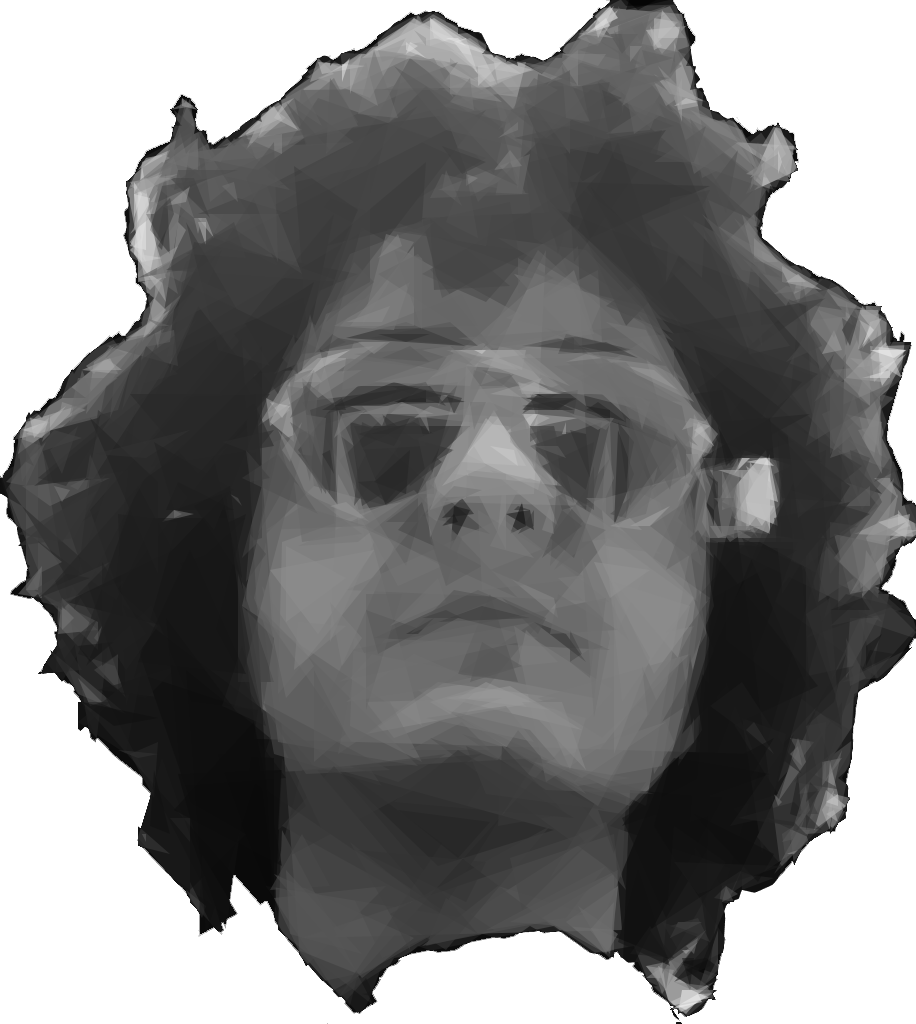
\includegraphics [width=2in] {2C-SE.assets/output1000.png}
\end{center}

\tableofcontents
\newpage

\hypertarget{18-september-2018}{%
\subsection{18 September 2018}\label{18-september-2018}}

\hypertarget{software-engineering-activities}{%
\subsubsection{Software Engineering
Activities}\label{software-engineering-activities}}

\begin{enumerate}
\def\labelenumi{\arabic{enumi}.}
\tightlist
\item
  Requirements Capture
\item
  Design
\item
  Construction/Implementation
\item
  Testing \& Debugging
\item
  Maintenance/Evolution
\end{enumerate}

\hypertarget{4-october-2018}{%
\subsection{4 October 2018}\label{4-october-2018}}

\hypertarget{identifying-classes-and-operations}{%
\subsubsection{Identifying Classes and
Operations}\label{identifying-classes-and-operations}}

\begin{itemize}
\item
  Identifying Classes

  \begin{itemize}
  \tightlist
  \item
    Ignore all non-nouns and instead focus on the \emph{nouns} in the
    \emph{project description}.
  \end{itemize}
\item
  Identifying Operations
\item
  Focus on \emph{verbs} instead.
\end{itemize}

\textbf{In both cases, use your judgement again to eliminate some
concepts for further simplicity and clarity.}

\textbf{Beware of subclassing/inheritance relationships between classes
(or of its concepts).}



\hypertarget{18-october-2018}{%
\subsection{18 October 2018}\label{18-october-2018}}

\hypertarget{software-configuration-management}{%
\subsubsection{Software Configuration
Management}\label{software-configuration-management}}

\begin{itemize}
\tightlist
\item
  Version Control
\item
  Compiling (and \emph{Building} as a general idea)
\end{itemize}

\hypertarget{version-control}{%
\subsubsection{Version Control}\label{version-control}}

\begin{itemize}
\item
  Lock-Modify-Unlock Model \emph{{[}OLD{]}}

  \begin{itemize}
  \item
    Advantages

    \begin{itemize}
    \tightlist
    \item
      Very simple.
    \item
      Central source of truth.
    \end{itemize}
  \item
    Disadvantages

    \begin{itemize}
    \tightlist
    \item
      Multiple developers cannot work on the same file.
    \item
      Deadlocks might occur (especially if scripts are doing some
      maintenance work on the repo for instance, say linting multiple
      files).
    \item
      Requires access to repo at all times (\emph{e.g.} you cannot
      checkout a file to modify it during the holiday, lest it will be
      inaccessible for a week).
    \end{itemize}
  \end{itemize}
\item
  Copy-Modify-Merge \emph{{[}NEW{]}}

  \begin{itemize}
  \item
    Advantages

    \begin{itemize}
    \tightlist
    \item
      Multiple developers can work on the same file at the same time.
    \item
      Deadlocks cannot occur since there is no locking.
    \item
      Distributed repositories might be beneficial for certain
      development. models (\emph{i.e.} open-source projects where every
      contributor might want to have a full-access).
    \item
      Does not require access to repo at all times.
    \end{itemize}
  \item
    Disadvantages

    \begin{itemize}
    \tightlist
    \item
      More complicated than Lock-Modify-Unlock model.
    \item
      Multiple sources of truth (though in reality there is often a
      master repo).
    \item
      Merge conflicts happen, and they are not uncommon.
    \item
      Automatic merging used to be faulty sometimes but software are
      getting better.
    \item
      Not every file-type is \emph{mergable}, such as photographs, PDF
      documents, audio files, or spreadsheets.

      \begin{itemize}
      \tightlist
      \item
        \textbf{Merging requires certain assumptions about the file
        semantics.}
      \end{itemize}
    \end{itemize}
  \end{itemize}
\end{itemize}



\begin{itemize}
\item
  Three-Way Merge

  \begin{enumerate}
  \def\labelenumi{\arabic{enumi}.}
  \item
    Original File:

\begin{verbatim}
Alpha
Bravo
Charlie
\end{verbatim}
  \item
    Tester 1 edits the Original File:

\begin{verbatim}
Alpha
Foxtrott
Charlie
\end{verbatim}
  \item
    Tester 2 edits the Original File:

\begin{verbatim}
Delta
Alpha
Echo
Charlie
\end{verbatim}
  \item
    Tester 2 commits changes.
  \item
    Tester 1's commit fails.
  \item
    Tester 1 updates and merge reports conflicts:

\begin{verbatim}
Delta
Alpha
<<<<<< .mine
Foxtrott
======
Echo
>>>>>> .r4
Charlie
\end{verbatim}
  \item
    Tester 1 now has to choose whether to retain her or Tester 2's
    version.
  \end{enumerate}
\end{itemize}

\hypertarget{compiling-and-building}{%
\subsubsection{Compiling and Building}\label{compiling-and-building}}

\begin{itemize}
\item
  C

  \begin{itemize}
  \tightlist
  \item
    Make \emph{{[}OLD{]}}
  \item
    CMake \emph{{[}NEW{]}}
  \end{itemize}
\item
  Java

  \begin{itemize}
  \tightlist
  \item
    Ant \emph{{[}OLD{]}}
  \item
    Maven \emph{{[}NEW{]}}
  \end{itemize}
\end{itemize}

\hypertarget{23-october-2018}{%
\subsection{23 October 2018}\label{23-october-2018}}

\hypertarget{refactoring}{%
\subsubsection{Refactoring}\label{refactoring}}

\begin{itemize}
\item
  \textbf{As code evolves its quality naturally decays.}

  \begin{itemize}
  \tightlist
  \item
    Because \textbf{changes are often local, without full understanding
    of the context.}
  \end{itemize}
\item
  \textbf{Refactoring}, is about restoring good design in a
  \emph{disciplined way}.

  \begin{itemize}
  \tightlist
  \item
    There are \textbf{refactoring patterns}.

    \begin{itemize}
    \tightlist
    \item
      There are patterns for everything in Software Engineering...
    \end{itemize}
  \end{itemize}
\item
  \emph{Refactoring is changing \textbf{internal} structure of software
  to make it:}

  \begin{itemize}
  \tightlist
  \item
    \emph{easier to understand, and}
  \item
    \emph{cheaper to modify}
  \end{itemize}

  \emph{\textbf{without changing its observable behaviour.}}
\item
  Refactoring was once seen as a kind of maintenance, but it can also be
  an integral part of the development process!

  \begin{itemize}
  \tightlist
  \item
    Agile methodologies (\emph{e.g.} XP) advocate continual refactoring.
  \end{itemize}
\item
  \textbf{A refactoring is a \emph{small} transformation.}

  \begin{itemize}
  \tightlist
  \item
    Do NOT confuse it with \textbf{rewrite}.
  \end{itemize}
\item
  To ensure that refactoring hasn't \textbf{changed}/broken something?

  \begin{itemize}
  \tightlist
  \item
    \emph{test, refactor, test}
  \end{itemize}
\end{itemize}

\hypertarget{bad-code-smells}{%
\subsubsection{Bad Code Smells}\label{bad-code-smells}}

\begin{itemize}
\tightlist
\item
  Duplicated code
\item
  Long methods
\item
  Large classes
\item
  Long parameter lists
\item
  Lazy classes \emph{i.e.} Classes that are ridiculously small.
\item
  Long message chains \emph{i.e.} Having too many (unnecessary)
  indirections.
\end{itemize}

\hypertarget{25-october-2018}{%
\subsection{25 October 2018}\label{25-october-2018}}

\hypertarget{verification-validation-and-testing-vvt}{%
\subsubsection{Verification, Validation, and Testing
(VV\&T)}\label{verification-validation-and-testing-vvt}}

\begin{itemize}
\tightlist
\item
  \textbf{VV\&T} generally refers to all techniques for improving
  \textbf{product quality}.
\item
  \textbf{Verification:} are we building the software \emph{right}?

  \begin{itemize}
  \tightlist
  \item
    Does software meet requirements?
  \item
    \emph{Static analysis, reviews, inspections, walk-throughs}
  \end{itemize}
\item
  \textbf{Validation:} are we building the \emph{right software}?

  \begin{itemize}
  \tightlist
  \item
    Does software accommodate customers' needs?
  \item
    \emph{Prototyping, early releases}
  \item
    Validation is more general than verification.
  \end{itemize}
\item
  \textbf{Testing is a useful technique for both.}
\end{itemize}

\hypertarget{testing}{%
\subsubsection{Testing}\label{testing}}

\begin{itemize}
\tightlist
\item
  In essence, testing is

  \begin{itemize}
  \tightlist
  \item
    \emph{Generating stimulus} for a component
  \item
    \emph{Collecting outputs} from the component
  \item
    \emph{Checking} if \emph{actual} outputs are as \emph{expected}
  \end{itemize}
\item
  \textbf{Automation of tests is essential.}

  \begin{itemize}
  \tightlist
  \item
    Speeds up the whole testing process.
  \item
    \textbf{Makes tests deterministic.}

    \begin{itemize}
    \tightlist
    \item
      Not necessarily always, but definitely more deterministic than a
      human being.
    \end{itemize}
  \end{itemize}
\item
  \texttt{assert} statements are common to compare the actual results
  and expectations.

  \begin{itemize}
  \tightlist
  \item
    \textbf{Checks can also be spread throughout the program code
    itself.}
  \end{itemize}
\end{itemize}

\hypertarget{kinds-of-tests}{%
\paragraph{Kinds of Tests}\label{kinds-of-tests}}

\begin{itemize}
\tightlist
\item
  Testing approaches:

  \begin{itemize}
  \tightlist
  \item
    \textbf{Black-Box Testing} purely specification-based (treating the
    component as a "black box")
  \item
    \textbf{White-Box Testing} also considers the internal structure
  \end{itemize}
\item
  Kinds of tests:

  \begin{itemize}
  \tightlist
  \item
    \textbf{Module (or Unit) Tests} for each class in OO software
  \item
    \textbf{Integration Tests} test components interact properly
  \item
    \textbf{System Tests} check if functional and non-functional
    requirements met, \emph{verification}
  \item
    \textbf{Acceptance Tests} in customer environment, \emph{validation}
  \item
    \textbf{Stress Tests} look for graceful degradation, not catastrophe
  \item
    \textbf{Performance Tests} performance is often a non-functional
    requirements (\emph{e.g.} in real-time systems)
  \item
    \textbf{Regression Tests} more like a testing methodology, repeated
    full-tests after each modification
  \end{itemize}
\end{itemize}

\hypertarget{how-to-test}{%
\paragraph{How to Test}\label{how-to-test}}

\begin{itemize}
\tightlist
\item
  Tests should be

  \begin{itemize}
  \tightlist
  \item
    \textbf{repeatable}
  \item
    \textbf{documented} both the tests and the results
  \item
    \textbf{precise}
  \item
    \textbf{done on configuration-controlled software}
  \end{itemize}
\item
  \textbf{Ideally test spec should be written at the same time as the
  requirements spec.}

  \begin{itemize}
  \tightlist
  \item
    Tests and requirement features can be cross-referenced!
  \item
    Use cases can suggest tests.
  \item
    \textbf{Also helps to ensure \emph{testability} of requirements.}
  \end{itemize}
\end{itemize}

\hypertarget{preconditions-postconditions-invariants}{%
\subsubsection{Preconditions, Postconditions,
Invariants}\label{preconditions-postconditions-invariants}}

\begin{itemize}
\tightlist
\item
  \textbf{Method Precondition} A condition that must be true when a
  method is invoked.
\item
  \textbf{Method Postcondition} A condition that the method guarantees
  to be true when it finishes.
\item
  \textbf{Class Invariant} A condition that should \emph{always} be true
  for all the instances of a given class.

  \begin{itemize}
  \tightlist
  \item
    \emph{Always} as in all \emph{client-visible} states, that is,
    whenever the object is not executing one of its methods!
  \end{itemize}
\end{itemize}

\hypertarget{java-modelling-language-jml}{%
\paragraph{Java Modelling Language
(JML)}\label{java-modelling-language-jml}}

\begin{itemize}
\item
  JML provides

  \begin{itemize}
  \tightlist
  \item
    A richer language (predicate logic) for writing boolean conditions
    than Java boolean expressions (propositional logic), for example
    allowing \emph{quantifiers} such as \texttt{\textbackslash{}forall}
    and \texttt{\textbackslash{}exists}.
  \item
    Special comment syntax for common assertion types:

    \begin{itemize}
    \tightlist
    \item
      \textbf{Preconditions:}
      \texttt{//@\ requires\ x\ \textgreater{}\ 0;}
    \item
      \textbf{Postconditions:}
      \texttt{//@\ ensures\ \textbackslash{}result\ \%\ 2\ ==\ 0;}
    \item
      \textbf{Invariants:}
      \texttt{//@invariant\ name.length\ \textless{}=\ 8;\ }
    \item
      \textbf{General assertions:} \texttt{//@\ assert\ i\ +\ j\ =\ 12;}
    \end{itemize}
  \end{itemize}
\item
  Examples:

  \begin{itemize}
  \item
\begin{Shaded}
\begin{Highlighting}[]
\CommentTok{//@ requires x >= 0.0}
\CommentTok{/*@ ensures JMLDouble}
\CommentTok{  @         .approximatelyEqualTo}
\CommentTok{  @        (x, \textbackslash{}result * \textbackslash{}result, eps);}
\CommentTok{  @*/}
\KeywordTok{public} \DataTypeTok{static} \DataTypeTok{double} \FunctionTok{sqrt}\NormalTok{(}\DataTypeTok{double}\NormalTok{ x) \{}
    \CommentTok{/*...*/}
\NormalTok{\}}
\end{Highlighting}
\end{Shaded}
  \item
\begin{Shaded}
\begin{Highlighting}[]
\CommentTok{/*@ requires a != null}
\CommentTok{  @       && (\textbackslash{}forall int i;}
\CommentTok{  @               0 < i && i < a.length;}
\CommentTok{  @               a[i-1] <= a[i]);}
\CommentTok{  @*/}
\DataTypeTok{int} \FunctionTok{binarySearch}\NormalTok{(}\DataTypeTok{int}\NormalTok{[] a, }\DataTypeTok{int}\NormalTok{ x) \{}
    \CommentTok{// ...}
\NormalTok{\}}
\end{Highlighting}
\end{Shaded}

    \begin{itemize}
    \item
      \begin{quote}
      Note that this universally quantified expression in JML must have
      parentheses around it, \texttt{(\textbackslash{}forall\ ...\ )}.
      \end{quote}
    \item
      \begin{quote}
      The range is optional, but if omitted, such a universally
      quantified expression may not be executable; it can still be used
      for documentation purposes, however.
      \end{quote}
    \end{itemize}
  \end{itemize}
\item
  \begin{quote}
  In return for the benefit of faster understanding, modular reasoning
  imposes a cost. This cost is that clients are not allowed to conclude
  anything that is not justified by the contracts of the methods that
  they call. Another way of looking at this is that, to allow modular
  reasoning with contract specifications, \textbf{the client code must
  work for every implementation that satisfies the contract.}
  \end{quote}

  \begin{itemize}
  \item
    \begin{quote}
    Otherwise, the implementation would no longer be free to change the
    algorithm used.
    \end{quote}
  \end{itemize}
\item
  \begin{quote}
  There are other good reasons not to use code as contracts.
  \textbf{Code makes a poor contract, because by only using code one
  cannot convey to readers what is intended (i.e., what the
  \emph{essential properties} of the method are) and what parts are
  merely implementation decisions (\emph{accidental features}).}
  \end{quote}

  \begin{itemize}
  \item
    \begin{quote}
    For example, if the code for \texttt{sqrt} computes square roots to
    7 decimal places, cannot this be changed in the next release?
    Without some separate description of what is intended, the reader
    can't tell if that 7 decimal places were intended, or just happened
    to be computed; perhaps 4 decimal places are all that is necessary
    for the rest of the program.
    \end{quote}
  \end{itemize}
\item
  Some tools such as \emph{jmlc, jmlrac, etc.} compile and run
  JML-annotated Java code into bytecode with specific \textbf{runtime
  assertion checking}.
\item
  \textbf{Assertions can also be used on \emph{inputs} to
  \emph{constrain} the \emph{random generation of input data}.}

  \begin{itemize}
  \tightlist
  \item
    QuickCheck!
  \end{itemize}
\end{itemize}

\emph{Quotes from:}
\href{http://www.eecs.ucf.edu/~leavens/JML//jmldbc.pdf}{http://www.eecs.ucf.edu/\textasciitilde{}leavens/JML//jmldbc.pdf}

\hypertarget{kinds-of-bugs}{%
\subsubsection{Kinds of Bugs}\label{kinds-of-bugs}}

\begin{itemize}
\item
  In order of increasing severity:

  \begin{enumerate}
  \def\labelenumi{\arabic{enumi}.}
  \tightlist
  \item
    \textbf{Mistake} A human action that produces a fault.
  \item
    \textbf{Fault (Defect)} An incorrect step, process, or data
    definition in a computer program.
  \item
    \textbf{Error} A difference between some computed value and the
    correct value.
  \item
    \textbf{Failure} The software (or whole system) failing to deliver
    some service it is expected to deliver.
  \end{enumerate}

  \begin{itemize}
  \tightlist
  \item
    \textbf{Faults do not necessarily lead to errors.}
  \item
    \textbf{Errors do not necessarily lead to failures.}
  \end{itemize}
\end{itemize}

\hypertarget{test-first-development}{%
\subsubsection{Test-First Development}\label{test-first-development}}

\begin{itemize}
\item
  \textbf{Motivation:} Tests implicitly define...

  \begin{itemize}
  \tightlist
  \item
    interface, and
  \item
    \textbf{specification of behaviour}
  \end{itemize}

  for the functionality being developed.
\item
  \textbf{Writing tests first often clarifies requirements!}

  \begin{itemize}
  \tightlist
  \item
    Testing code demands more precision than an English specification.
  \end{itemize}
\item
  \textbf{Idea} is

  \begin{itemize}
  \tightlist
  \item
    write tests \textbf{before} writing the code they apply to,
  \item
    run tests as code is written.
  \item
    \emph{In an ideal world, the system will be complete when all your
    tests pass. :)}
  \item
    \textbf{TFD avoids poor ambiguity resolution.}

    \begin{itemize}
    \tightlist
    \item
      Instead of choosing what is easiest to implement in the face of
      ambiguity, you will implement the right thing (that your tests
      check for).
    \end{itemize}
  \end{itemize}
\item
  \textbf{Consequently}

  \begin{itemize}
  \tightlist
  \item
    bugs found at earliest possible point of development
  \item
    locating bugs are relatively easy (due to locality of tests)
  \item
    \textbf{TFD ensures adequate time for test writing.}

    \begin{itemize}
    \tightlist
    \item
      Often testing time is squeezed or eliminated.
    \end{itemize}
  \end{itemize}
\end{itemize}

\hypertarget{test-driven-development}{%
\subsubsection{Test-Driven Development}\label{test-driven-development}}

\begin{itemize}
\tightlist
\item
  A subtly different term, covers the way that in Extreme Programming
  detailed tests \emph{replace} a written specification.
\end{itemize}

\hypertarget{limitations-of-testing}{%
\subsubsection{Limitations of Testing}\label{limitations-of-testing}}

\begin{itemize}
\item
  \textbf{Writing tests is time-consuming}
\item
  \textbf{Coverage almost always limited} may happen not to exercise a
  bug.
\item
  \textbf{Difficult/impossible to emulate live environment perfectly}
  \emph{e.g.} \emph{race conditions} that appear under real load
  conditions can be hard to find by testing.
\item
  \textbf{Can only test executable things} mainly code, or certain kinds
  of model -- not high level design or requirements.
\end{itemize}

\hypertarget{reviews-walkthroughs-inspections}{%
\subsubsection{Reviews, Walkthroughs,
Inspections}\label{reviews-walkthroughs-inspections}}

\begin{itemize}
\tightlist
\item
  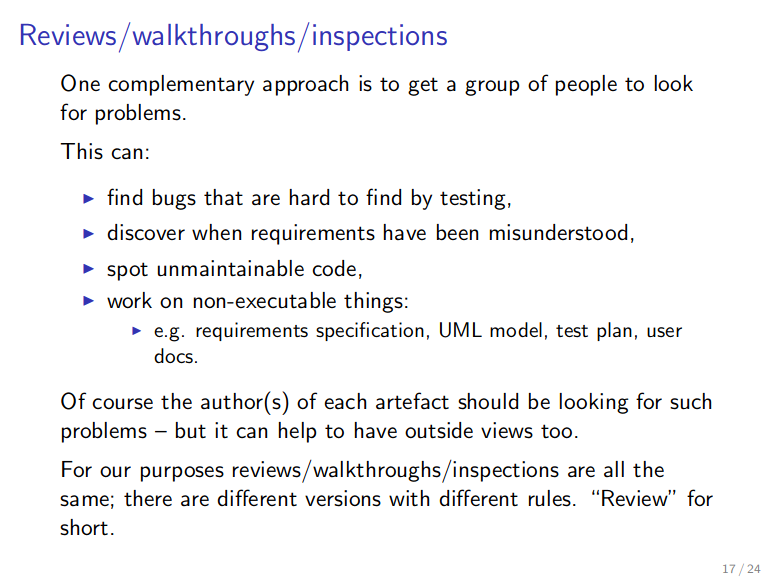
\includegraphics{2C-SE.assets/1542636369213.png}
\item
  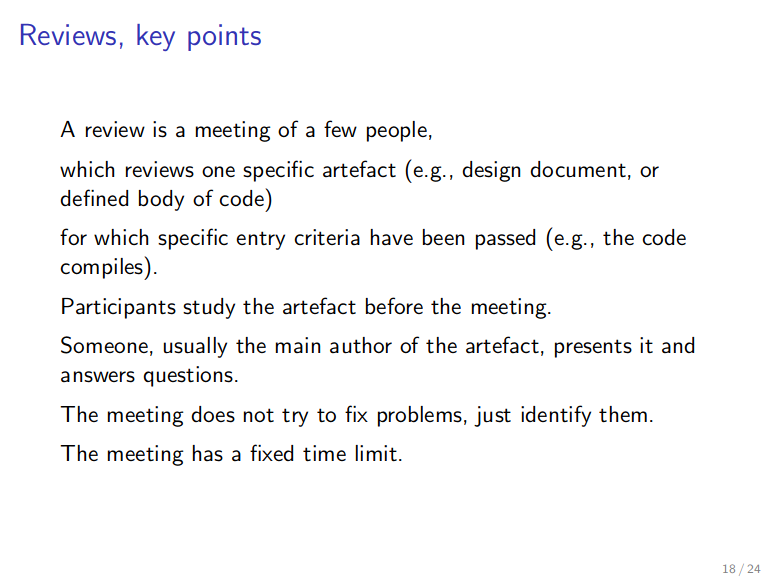
\includegraphics{2C-SE.assets/1542636375661.png}
\end{itemize}

\hypertarget{static-analysis}{%
\subsubsection{Static Analysis}\label{static-analysis}}

\begin{itemize}
\tightlist
\item
  Static analysis is \textbf{the inspection of the code to determine
  properties of it \emph{without running it}.}

  \begin{itemize}
  \tightlist
  \item
    When contrasted with testing, testing is called \emph{dynamic
    testing}.
  \end{itemize}
\item
  \textbf{Type-checking} during compilation is a basic kind of static
  analysis.
\item
  \textbf{Trade-offs}

  \begin{itemize}
  \tightlist
  \item
    As the properties checked get more complicated,

    \begin{itemize}
    \tightlist
    \item
      only smaller programs can be analysed.
    \item
      the process is less automated (\emph{e.g.} \textbf{annotations}
      required).
    \end{itemize}
  \item
    As tools are more automated and designed to work on larger programs,
    they often \emph{cannot}

    \begin{itemize}
    \tightlist
    \item
      guarantee every problem flagged is a real error (\emph{i.e.}
      false-positives)
    \item
      find every error (\emph{i.e.} false-negatives).
    \end{itemize}
  \item
    The latter kind of tools are more to aid bug-hunting than ensuring
    \emph{correctness}.
  \end{itemize}
\end{itemize}

\hypertarget{1-november-2018}{%
\subsection{1 November 2018}\label{1-november-2018}}

\hypertarget{deployment}{%
\subsubsection{Deployment}\label{deployment}}

\begin{itemize}
\tightlist
\item
  Getting software out of the hands of the developers into the hands of
  the users.
\item
  More than 50\% of commissioned software is not used, mostly because it
  fails at deployment stage.
\end{itemize}

\hypertarget{key-issues}{%
\paragraph{Key Issues}\label{key-issues}}

\begin{itemize}
\item
  \textbf{Business processes} Most large software systems require the
  customer to change the way they work; has this been properly thought
  through?
\item
  \textbf{Training}
\item
  \textbf{Deployment itself} How \emph{physically} to get the software
  installed.
\item
  \textbf{Equipment} Is the customers' hardware up to the job?
\item
  \textbf{Expertise} Does the customer have the IT expertise to install
  \& use the software?
\item
  \textbf{Integration} How will the software integrate with other
  systems of the customers'?
\item
  "Installing" is the easiest part of deployment...
\end{itemize}

\hypertarget{maintenance}{%
\subsubsection{Maintenance}\label{maintenance}}

The process of \emph{changing a system after it has been delivered}.

\begin{itemize}
\tightlist
\item
  \textbf{Fixing bugs and vulnerabilities} not only in code, but also
  design and requirements
\item
  \textbf{Adapting to new platforms and software environments}
  \emph{e.g.} new hardware, new OSes, new software/systems to
  integrate...
\item
  \textbf{Supporting new features and requirements} necessary as
  operating environments change in response to competitive pressures.
\end{itemize}

\hypertarget{challanges}{%
\paragraph{Challanges}\label{challanges}}

\begin{itemize}
\tightlist
\item
  \textbf{(Un)popularity of maintenance work:}

  \begin{itemize}
  \tightlist
  \item
    Unpopular -\/- seen as less skilled, can (and often does) involve
    obsolete languages.
  \end{itemize}
\item
  Often a new team has to understand the software.
\item
  \textbf{Development and maintenance often separate business
  contracts.}
\item
  Things often degrade over time.
\item
  Working with obsolete compilers, OSes, hardware...
\end{itemize}

\hypertarget{re-engineering}{%
\subsubsection{Re-engineering}\label{re-engineering}}

\begin{itemize}
\tightlist
\item
  \textbf{Source code translation} \emph{E.g.} from obsolete language,
  or assembly, to modern language, ...
\item
  \textbf{Reverse engineering} \emph{I.e.} analysing the program,
  possibly in the absence of source code!
\item
  \textbf{Structure improvement} Especially modularisation,
  architectural refactoring, ...
\item
  \textbf{Data re-engineering} Reformatting and cleaning up data.
\item
  \textbf{Adding adaptor interfaces \textless{}3} to users and newer
  other software
\end{itemize}

\hypertarget{issues}{%
\paragraph{Issues}\label{issues}}

\begin{itemize}
\tightlist
\item
  Specification might be lost as well...
\item
  Which bugs do you deliberately preserve?
\end{itemize}

\hypertarget{bug-reporting}{%
\subsubsection{Bug Reporting}\label{bug-reporting}}

\begin{itemize}
\item
  Many projects use a \emph{bug tracking system} for both bug reports
  and new feature requests.
\item
  These provide extensive support for \emph{receiving}, \emph{tracking},
  notifying, monitoring, \emph{etc.}
\item
  Each \emph{ticket} has a

  \begin{itemize}
  \tightlist
  \item
    unique \textbf{ticket number}
  \item
    \textbf{summary}
  \item
    \textbf{component} where the bug is observed (it might not always be
    clear; sometimes bugs arise out of integration issues)
  \item
    \textbf{version} of the program
  \item
    \textbf{milestone} in which this bug is aimed to be fixed
  \item
    \textbf{type} \emph{e.g.} \emph{defect}, or maybe \emph{enhancement}
    for feature requests!
  \item
    \textbf{owner} \emph{i.e.} the creator of the ticket
  \item
    \textbf{assignee} \emph{i.e.} the person responsible for the
    resolution of the ticket
  \item
    \textbf{status} \emph{new}, \emph{assigned}, \emph{notabug} if the
    developers think it's not a bug, \emph{resolved}, ...
  \item
    \textbf{priority} some bugs and/or feature requests are more
    important than others!
  \item
    and much more!
  \end{itemize}
\item
  When \textbf{reporting bugs}:

  \begin{itemize}
  \tightlist
  \item
    Include tediously detailed information about

    \begin{itemize}
    \tightlist
    \item
      what \emph{exactly} you did

      \begin{itemize}
      \tightlist
      \item
        so that bug can be \emph{reproduced}
      \end{itemize}
    \item
      what did you expect to happen
    \item
      what happened instead
    \end{itemize}
  \item
    Include full information about the system \& environment such as

    \begin{itemize}
    \tightlist
    \item
      operating system
    \item
      hardware (processor, graphics card, ...)
    \end{itemize}
  \item
    Make an intelligent attempt at diagnosing the problem if you can.

    \begin{itemize}
    \tightlist
    \item
      Keep your \emph{diagnosis} completely separate from the report of
      \emph{what happened}.
    \end{itemize}
  \item
    Add a concise summary at the beginning.
  \item
    Do \textbf{not} omit information you think is irrelevant; you are
    probably wrong in what you think.
  \end{itemize}
\end{itemize}

\hypertarget{8-november-2018}{%
\subsection{8 November 2018}\label{8-november-2018}}

\hypertarget{software-processes}{%
\subsubsection{Software Processes}\label{software-processes}}

\begin{itemize}
\tightlist
\item
  A process is \emph{"a set of activities and way of
  organising/coordinating those activities in order to produce a
  software system."}
\item
  \textbf{Activities:}

  \begin{itemize}
  \tightlist
  \item
    \textbf{Software Specification} goals, functionality, and
    constraints
  \item
    \textbf{Software Development} producing software: design,
    construction, verification
  \item
    \textbf{Software Validation} ensuring that software accommodates the
    customers' needs
  \item
    \textbf{Software Evolution} adapting software to changing needs and
    requirements
  \end{itemize}
\item
  Processes are about \emph{management}:

  \begin{itemize}
  \tightlist
  \item
    ordering activities
  \item
    outcomes of activities
  \item
    allocating people and resources
  \item
    planning in advance, predicting time/cost/resource usage
  \item
    \textbf{monitoring}
  \item
    \textbf{risk reduction}
  \end{itemize}
\item
  \textbf{Process models} are \emph{ideals}, in practice mix and match!
\end{itemize}

\hypertarget{waterfall-model}{%
\paragraph{Waterfall Model}\label{waterfall-model}}

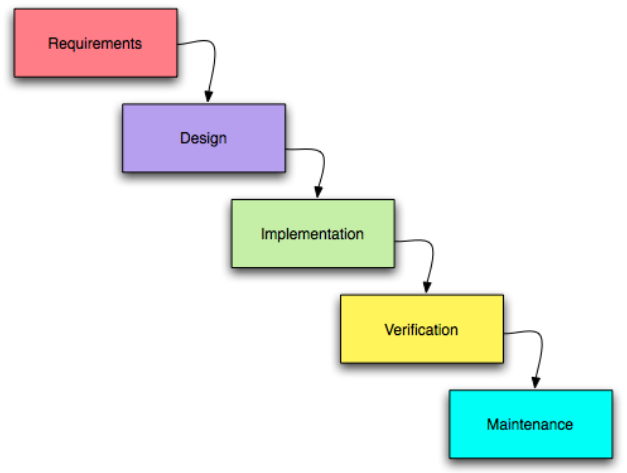
\includegraphics{2C-SE.assets/1543142448637.png}

\textbf{Pros:}

\begin{itemize}
\tightlist
\item
  Better than no process at all, makes clear that requirements must be
  analysed, software must be tested, \emph{etc.}
\item
  Suitable for

  \begin{itemize}
  \tightlist
  \item
    very slowly evolving systems where high-reliability, safety
    \emph{etc.} are top priorities (\emph{e.g.} engine control unit of a
    car), in other words, \textbf{safety-critical}
  \item
    for \textbf{embedded systems} where resources are extremely limited
    and deployment is often only once (during flashing!),
  \item
    very \textbf{large systems} where the interaction between multiple
    components must be clearly laid out (which also allows simultaneous
    development of different components).
  \end{itemize}
\end{itemize}

\textbf{Cons:}

\begin{itemize}
\tightlist
\item
  Inflexible and unrealistic: \emph{e.g.} verification will show up
  problems with requirements capture.

  \begin{itemize}
  \tightlist
  \item
    Many real-world application (need to) evolve rapidly in response to
    the changing customer needs and competitive market conditions.
  \end{itemize}
\item
  Slow and expensive: in an attempt to avoid problems later, we end up
  "gold plating" early phases.

  \begin{itemize}
  \tightlist
  \item
    \emph{E.g.} Over-engineering at Requirements and Design stage so to
    avoid problems during implementation and verification.
  \end{itemize}
\end{itemize}

\hypertarget{spiral-model}{%
\paragraph{Spiral Model}\label{spiral-model}}

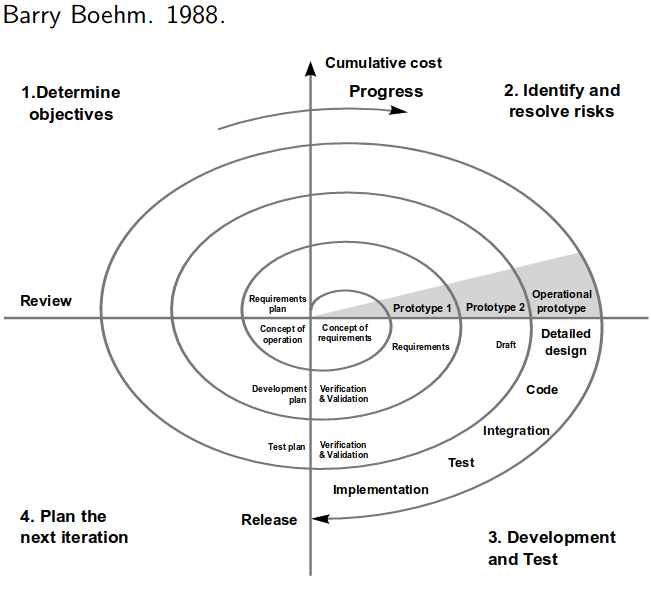
\includegraphics{2C-SE.assets/1543143069292.png}

\begin{itemize}
\tightlist
\item
  \textbf{Cycles} are an essential concept:

  \begin{enumerate}
  \def\labelenumi{\arabic{enumi}.}
  \tightlist
  \item
    Determine \textbf{Objectives} objectives are settled
  \item
    Identify and Resolve \textbf{Risks} risks identified, alternatives
    considered (\emph{e.g.} go for prototype to analyse uncertain
    requirements)
  \item
    \textbf{Development and Test}
  \item
    \textbf{Review} for the next iteration project reviewed and
    decisions made about continuing
  \end{enumerate}
\item
  \textbf{A key innovation is prominent role of risk.}
\end{itemize}

\textbf{Pros:}

\begin{itemize}
\tightlist
\item
  Risk plays a prominent role, which is crucial.
\item
  Iterative approach is more suitable (than the Waterfall) to
  real-world.
\item
  Steps are clearly identified.
\end{itemize}

\textbf{Cons:}

\begin{itemize}
\tightlist
\item
  Loops are still \emph{sequential}, but in real-world it's more of a
  back-and-forth, and there is more concurrency (\emph{e.g.} realising
  that a requirement has been misunderstood during development forces
  you to revise your requirements)
\item
  Steps are not as elaborate as UP for instance; no guidelines on how to
  proceed with validation, with business modelling, and how the
  importance of each varies through the time...
\end{itemize}

\hypertarget{unified-process}{%
\paragraph{Unified Process}\label{unified-process}}

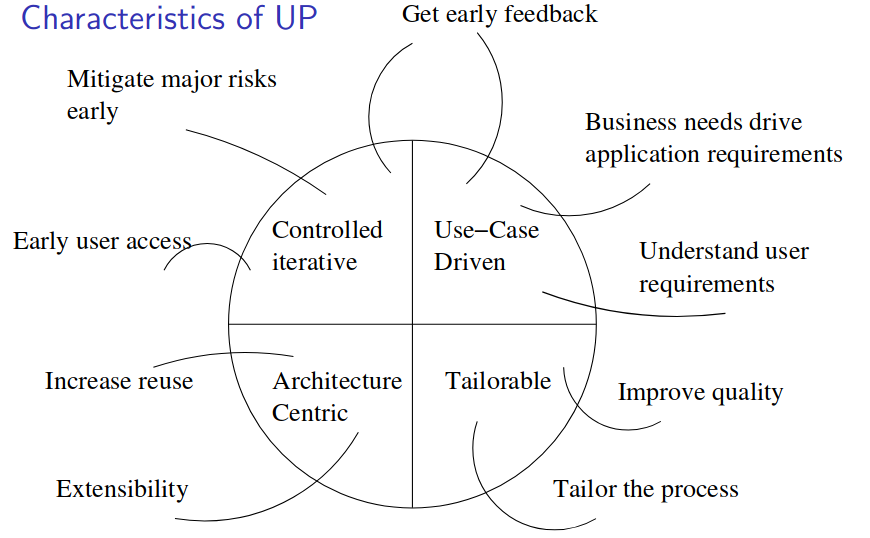
\includegraphics{2C-SE.assets/1543143798585.png}

\begin{itemize}
\tightlist
\item
  Again, \textbf{cycles}:

  \begin{enumerate}
  \def\labelenumi{\arabic{enumi}.}
  \tightlist
  \item
    \textbf{Inception} ends with commitment from the \emph{project
    sponsor} to go ahead: \emph{business case} for the project and its
    basic feasibility \& scope known
  \item
    \textbf{Elaboration} ends with

    \begin{itemize}
    \tightlist
    \item
      \textbf{basic architecture} of the system in place
    \item
      a \textbf{plan for construction} agreed
    \item
      all \textbf{significant risks identified}
    \end{itemize}
  \item
    \textbf{Construction} (definitely \textbf{iterative}) ends with a
    beta-release system
  \item
    \textbf{Transition} is introducing the system to its users
  \end{enumerate}
\item
  The process for a single product will have several \emph{cycles}.
\item
  \textbf{Each instance of a phase might have several iterations.}
\end{itemize}

\hypertarget{workflows}{%
\subparagraph{Workflows}\label{workflows}}

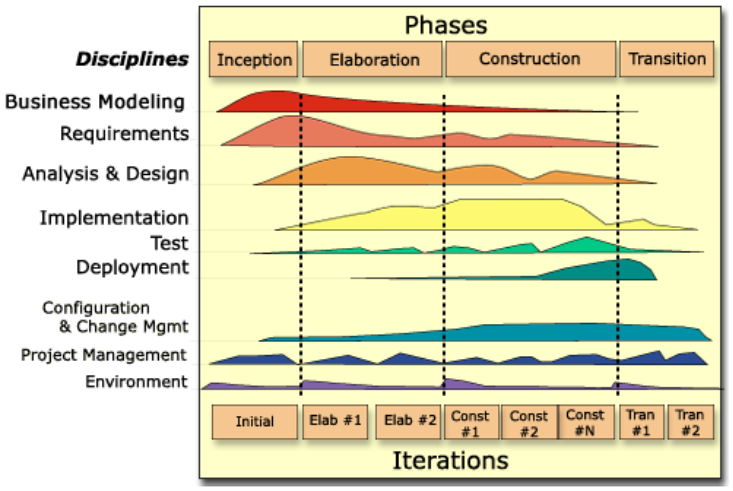
\includegraphics{2C-SE.assets/1543144642816.png}

\textbf{6 Engineering workflows:}

\begin{enumerate}
\def\labelenumi{\arabic{enumi}.}
\tightlist
\item
  \textbf{Business modelling} {[}Inception cycle{]} A key \emph{pro} of
  UP is the fact that it includes the \emph{business} side of software
  engineering into the software process itself. The fact that
  \emph{business modelling} precedes \emph{requirements} evidences that
  software is developed to serve a (business) purpose.
\item
  Requirements {[}Elaboration cycle{]}
\item
  Analysis and design {[}Elaboration cycle{]}
\item
  Implementation {[}Construction cycle{]}
\item
  Test {[}Construction cycle{]}
\item
  Deployment {[}Transition cycle{]}
\end{enumerate}

\textbf{3 Supporting workflows:} always ongoing workflows in the
background

\begin{enumerate}
\def\labelenumi{\arabic{enumi}.}
\tightlist
\item
  Configuration and change management
\item
  Project management
\item
  Environment (\emph{e.g.} process and tools)
\end{enumerate}

\hypertarget{up-best-practises}{%
\subparagraph{UP Best Practises}\label{up-best-practises}}

\begin{enumerate}
\def\labelenumi{\arabic{enumi}.}
\tightlist
\item
  \textbf{Develop software iteratively}
\item
  \textbf{Manage requirements} document explicitly, analyse impact
  before adopting
\item
  \textbf{Use component-based architectures} promote systematic reuse
\item
  \textbf{Visually model software} UML...
\item
  \textbf{Verify software quality} testing, linting, coding standards
\item
  \textbf{Control change to software} configuration management
\end{enumerate}

\hypertarget{personal-software-process}{%
\paragraph{Personal Software Process}\label{personal-software-process}}

\begin{itemize}
\item
  UNIMPORTANT.
\item
  \textbf{PSP provides a ladder of gradually more sophisticated
  practises.}
\item
  The idea:

  \begin{enumerate}
  \def\labelenumi{\arabic{enumi}.}
  \tightlist
  \item
    Identify those (UP) large-system \textbf{software methods \&
    practises that can be used by individuals},
  \item
    Define a subset of those methods and practises that can be applied
    while developing \textbf{small programs},
  \item
    Structure them so that they can \textbf{gradually introduced},
  \item
    Provide \textbf{exercises suitable for practising} these methods in
    an educational setting.
  \end{enumerate}
\item
  Lots of forms to fill in: time recording log, defect recording log,
  ...
\item
  A relatively \textbf{high ceremony} process, aimed at
  \textbf{individuals and small projects}.

  \begin{itemize}
  \tightlist
  \item
    It's often used as a training for high(er) ceremony processes such
    as UP.
  \end{itemize}
\end{itemize}

\hypertarget{13-november-2018}{%
\subsection{13 November 2018}\label{13-november-2018}}

\hypertarget{agile-processes}{%
\subsubsection{Agile Processes}\label{agile-processes}}

\begin{itemize}
\tightlist
\item
  Software development has to be \emph{agile}: \textbf{able to react
  quickly to change}
\item
  \textbf{Maxims:}

  \begin{itemize}
  \tightlist
  \item
    \textbf{Individuals and interactions} over processes and tools
  \item
    \textbf{Working software} over comprehensive documentation
  \item
    \textbf{Customer collaboration} over contract negotiation
  \item
    \textbf{Responding to change} over following a plan
  \end{itemize}
\end{itemize}

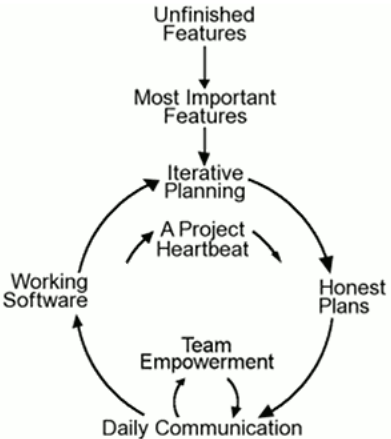
\includegraphics{2C-SE.assets/1543146629660.png}

\hypertarget{12-principles-of-agile}{%
\paragraph{12 Principles of Agile}\label{12-principles-of-agile}}

\begin{enumerate}
\def\labelenumi{\arabic{enumi}.}
\tightlist
\item
  \textbf{Customer satisfaction} by \textbf{rapid delivery} of
  \textbf{useful software}
\item
  \textbf{Welcome changing requirements}, even late in development
\item
  \textbf{Working software is delivered frequently (weeks rather than
  months)}
\item
  \textbf{Working software is the principal measure of progress}
\item
  \textbf{Sustainable development}, able to \textbf{maintain a constant
  pace}
\item
  \textbf{Close, daily co-operation between business people and
  developers}
\item
  Face-to-face conversation is the best form of communication
  (\textbf{co-location})
\item
  Projects are built around motivated \textbf{individuals, who should be
  given right support and trusted to get job done}
\item
  \textbf{Continuous attention} to technical excellence and good design
\item
  \textbf{Simplicity is essential}
\item
  Best requirements and designs form \textbf{self-organising teams}
\item
  \textbf{Regular reflection} on process and tuning of behaviour
\end{enumerate}

\hypertarget{extreme-programming-xp}{%
\subsubsection{Extreme Programming (XP)}\label{extreme-programming-xp}}

\begin{itemize}
\item
  \textbf{EXTREME PROGRAMMING IS AN AGILE VARIANT.}

  \begin{itemize}
  \tightlist
  \item
    Other Agile processes include Scrum and DSDM.
  \end{itemize}

  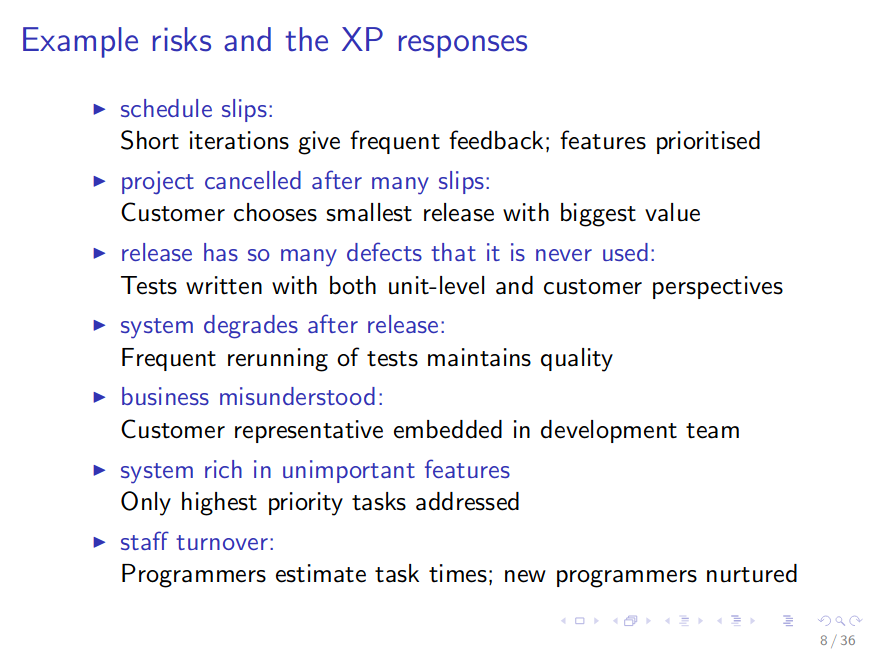
\includegraphics{2C-SE.assets/1543147108484.png}
\item
  \textbf{Activities}

  \begin{itemize}
  \tightlist
  \item
    \textbf{Listening} understanding the customer, communicating
    efficiently
  \item
    \textbf{Designing} creating structure, organising system logic
  \item
    \textbf{Coding}
  \item
    \textbf{Testing} \emph{embodying requirements}, assessing quality,
    guiding coding
  \end{itemize}
\end{itemize}

\hypertarget{xp-practices---planning-game}{%
\subparagraph{XP Practices - Planning
Game}\label{xp-practices---planning-game}}

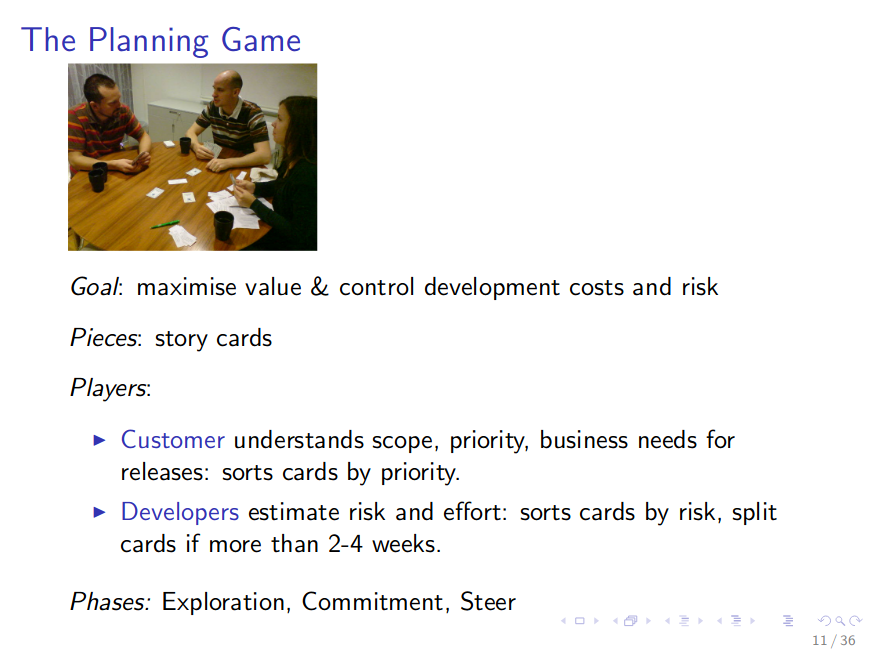
\includegraphics{2C-SE.assets/1543147264443.png}

\hypertarget{xp-practices---on-site-customer}{%
\subparagraph{XP Practices - On-Site
Customer}\label{xp-practices---on-site-customer}}

\begin{itemize}
\tightlist
\item
  Someone capable of making the business's decisions in the planning
  game, a representative of the customer who sits with the development
  team, being always ready to

  \begin{itemize}
  \tightlist
  \item
    clarify
  \item
    (help) write functional tests
  \item
    make small-scale priority and scope decisions
  \end{itemize}
\item
  Customer can do their \emph{normal work} when not needed to interact
  with the development team.
\end{itemize}

\hypertarget{xp-practices---small-releases}{%
\subparagraph{XP Practices - Small
Releases}\label{xp-practices---small-releases}}

\begin{itemize}
\tightlist
\item
  \textbf{Release as frequently as is possible whilst still adding some
  \emph{business value} in each release.}

  \begin{itemize}
  \tightlist
  \item
    \textbf{You get feedback as soon as possible.}
  \item
    \textbf{Lets the customer have the most essential functionality
    ASAP.}
  \end{itemize}
\item
  Every week or every month.
\item
  Outside XP releases commonly every 6 months or longer.
\end{itemize}

\hypertarget{xp-practices---methaphors}{%
\subparagraph{XP Practices -
Methaphors}\label{xp-practices---methaphors}}

\begin{itemize}
\tightlist
\item
  About an easily-communicated overarching view of the system.
\item
  \textbf{Encompasses concept of software architecture.}
\item
  \textbf{Eases the developer-customer communication.}
\item
  Provides a sense of cohesion.
\item
  \textbf{Often suggests a consistent vocabulary.}
\end{itemize}

\hypertarget{xp-practices---continuous-integration}{%
\subparagraph{XP Practices - Continuous
Integration}\label{xp-practices---continuous-integration}}

\begin{itemize}
\tightlist
\item
  \textbf{Code is integrated, debugged, and tested in full system build
  frequently} (at most a few hours or a day after being written).
\item
  \textbf{Maintains a working system at all times.}
\item
  \textbf{Makes bugs easier to trace.}

  \begin{itemize}
  \tightlist
  \item
    "It was alright an hour ago! Let me check what has changed since
    then."
  \end{itemize}
\item
  \textbf{Simplifies integration, prevents late-stage surprises.}
\end{itemize}

\hypertarget{xp-practices---testing}{%
\subparagraph{XP Practices - Testing}\label{xp-practices---testing}}

\begin{itemize}
\tightlist
\item
  \textbf{Any program feature without an automated test simply doesn't
  exist.}
\item
  \textbf{Tests are the contract between your developers, and between
  you and your customers.}

  \begin{itemize}
  \tightlist
  \item
    Programmers write \textbf{unit tests}.
  \item
    Customers (with your help) write \textbf{functional tests}.
  \end{itemize}
\end{itemize}

\hypertarget{xp-practices---refactoring}{%
\subparagraph{XP Practices -
Refactoring}\label{xp-practices---refactoring}}

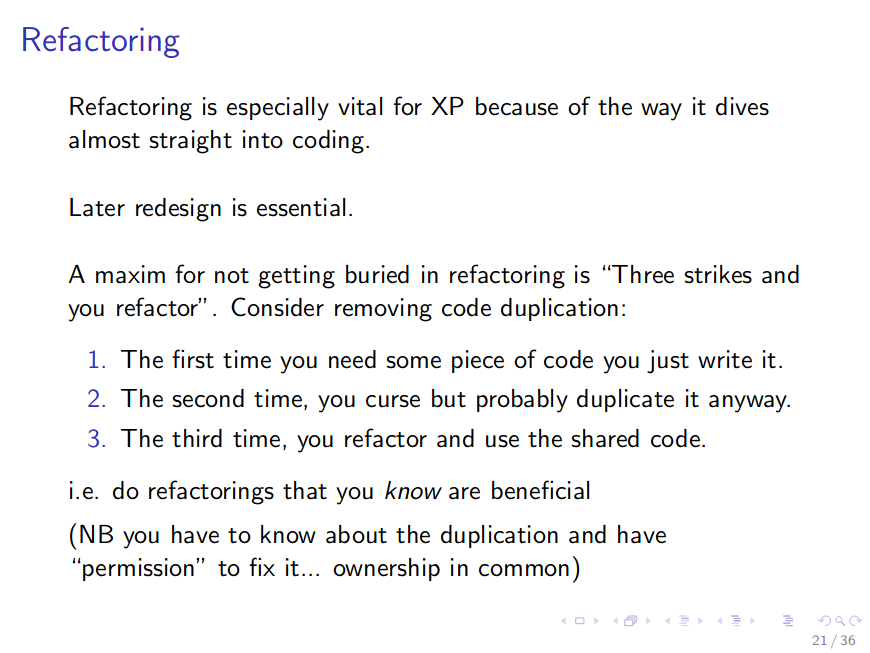
\includegraphics{2C-SE.assets/1543147982905.png}

\hypertarget{xp-practices---pair-programming}{%
\subparagraph{XP Practices - Pair
Programming}\label{xp-practices---pair-programming}}

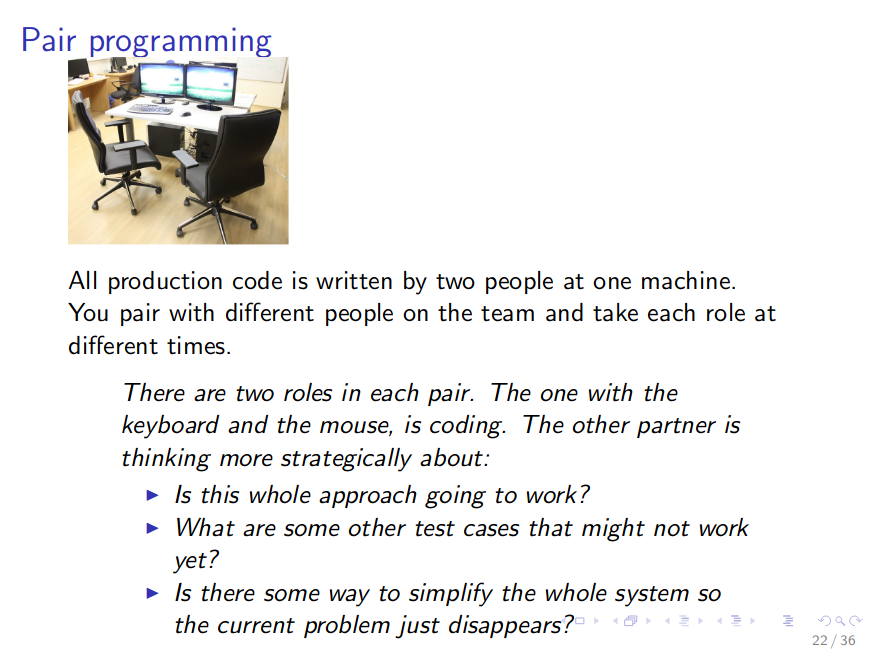
\includegraphics{2C-SE.assets/1543148029020.png}

\hypertarget{xp-practices---collective-ownership}{%
\subparagraph{XP Practices - Collective
Ownership}\label{xp-practices---collective-ownership}}

\begin{itemize}
\tightlist
\item
  \textbf{Every developer is responsible for the codebase as a whole},
  and is permitted to modify and improve as they seem fit.
\end{itemize}

\hypertarget{xp-practices---coding-standards}{%
\subparagraph{XP Practices - Coding
Standards}\label{xp-practices---coding-standards}}

\begin{itemize}
\tightlist
\item
  \textbf{The whole team adheres to a single set of \emph{conventions}
  about how code is written.}

  \begin{itemize}
  \tightlist
  \item
    \textbf{In order to make \emph{pair programming} and
    \emph{collective ownership} work.}
  \end{itemize}
\end{itemize}

\hypertarget{mixing-and-matching-xp-practices}{%
\subparagraph{Mixing and Matching XP
Practices}\label{mixing-and-matching-xp-practices}}

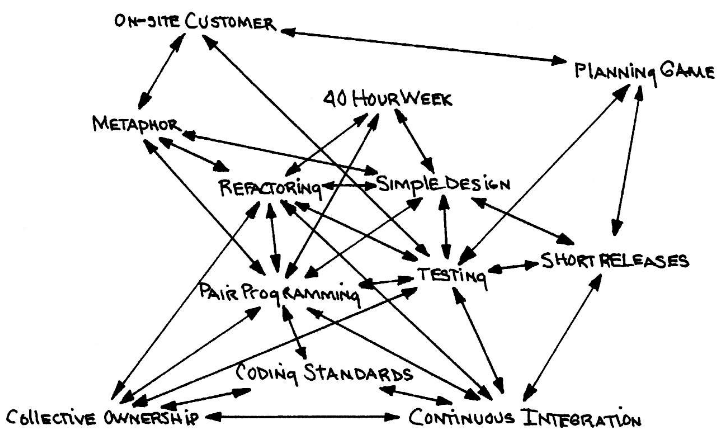
\includegraphics{2C-SE.assets/1543148331734.png}

\begin{itemize}
\tightlist
\item
  XP practices are \emph{very} interrelated \& interdependent so it's
  dangerous:

  \begin{itemize}
  \tightlist
  \item
    \emph{Collective Ownership} without \emph{Coding Standards} will
    create an inconsistent mess.
  \item
    \emph{Simple Design} without \emph{Refactoring} will create code
    smell.
  \item
    \emph{Planning Game} without \emph{On-Site Customer} is simply
    unimaginable!
  \end{itemize}
\end{itemize}

\hypertarget{comparison-of-different-processes}{%
\subsubsection{Comparison of Different
Processes}\label{comparison-of-different-processes}}

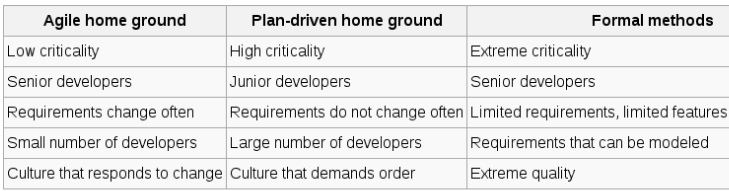
\includegraphics{2C-SE.assets/1543148442267.png}

\begin{itemize}
\tightlist
\item
  \textbf{Formal Methods} go beyond Waterfall and what we've seen in
  this course.

  \begin{itemize}
  \tightlist
  \item
    Developing on-board software for Curiosity Space Rover for instance!
  \end{itemize}
\end{itemize}

\hypertarget{15-november-2018}{%
\subsection{15 November 2018}\label{15-november-2018}}

\hypertarget{improving-processes}{%
\subsubsection{Improving Processes}\label{improving-processes}}

\hypertarget{risks}{%
\paragraph{"Risks"}\label{risks}}

\begin{itemize}
\tightlist
\item
  We improve a process to manage (\emph{i.e.} reduce, predict, and plan
  for) \textbf{risks} (\emph{i.e.} bad things that might happen to us).
\item
  \textbf{Risks can be categorised in many different ways.}

  \begin{itemize}
  \tightlist
  \item
    \textbf{Project risks} affect schedule or resources \emph{e.g.}
    staff loss, management change, missing resources
  \item
    \textbf{Product risks} affect quality or performance of the software
    \emph{e.g.} always-changing requirements, delays in requirements
    analysis (and consequently rushing it)
  \item
    \textbf{Business risks} affect the software developer or buyer
    \emph{e.g.} mis-estimation of costs, competitor gets to market first
  \end{itemize}
\item
  \textbf{Planing for risks}

  \begin{itemize}
  \tightlist
  \item
    \textbf{Identify} risks early, categorise them
  \item
    \textbf{Analyse} each identified risk; is it minor, major, serious,
    fatal? What is the \emph{chance} of it happening?
  \item
    \textbf{Plan} how to \emph{cope} with each risk:

    \begin{itemize}
    \tightlist
    \item
      Can it be \textbf{avoided} by reducing the probability of
      occurrence?
    \item
      Can you plan to \textbf{minimise} the effect if it does happen?
    \item
      What is your \textbf{contingency plan} if it does happen?
    \end{itemize}
  \end{itemize}
\end{itemize}

\hypertarget{quality}{%
\paragraph{"Quality"}\label{quality}}

\begin{itemize}
\item
  \textbf{Quality is anything that the customer cares about.}

  \begin{itemize}
  \tightlist
  \item
    \textbf{Quality planning} \emph{how will you ensure that this
    project delivers a high quality product?}
  \item
    \textbf{Quality metrics} \emph{what measurements must you make in
    order to tell whether what you're doing is making the difference you
    intend?}
  \item
    \textbf{Quality improvement} \emph{what can you learn from this
    project to help you plan and run the next one better?}
  \item
    \textbf{Quality control} \emph{how can you ensure and prove that
    your quality plan was followed?}
  \item
    \textbf{Quality assurance (QA)} \emph{an umbrella term for the whole
    field dealing with quality.}
  \end{itemize}
\item
  Quality improvement may focus on

  \begin{itemize}
  \tightlist
  \item
    \emph{the software product itself} verification, validation,
    testing, code/design reviews, inspections, walkthroughs...
  \item
    \emph{the process by which the software is produced} what we'll
    focus on!
  \end{itemize}
\item
  \textbf{Process focus}

  \begin{itemize}
  \tightlist
  \item
    {[}+{]} has the potential to improve \emph{all} products of the
    organisation
  \item
    {[}+{]} makes it possible to \emph{certify} (ISO 9000) the whole
    organisation
  \item
    {[}+{]} might be unavoidable as some things -\/-such as
    planning-\/-are hard to approach in any other way
  \item
    {[}-{]} done badly, can easily increase costs with no actual
    benefits
  \end{itemize}
\item
  \textbf{Centres of Process-Focused Quality Assurance}

  \begin{enumerate}
  \def\labelenumi{\arabic{enumi}.}
  \tightlist
  \item
    \textbf{Organisation -\/-\/-\textgreater{} Project
    -\/-\/-\textgreater{} Individual} Organisation's management
    \emph{decides}, influencing projects. Project managers \emph{direct}
    individuals into desired behaviour.
  \item
    \textbf{Organisation \textless{}-\/-\/- Project \textless{}-\/-\/-
    Individual} Individuals \emph{introduce} improvements to the rest of
    the project. Project improvements \emph{spread} to the rest of the
    organisation.
  \end{enumerate}

  \begin{itemize}
  \tightlist
  \item
    Making these centres work together productively depends on the
    software engineering \emph{culture} of the organisation and
    \emph{attitude to work} of the individual.
  \end{itemize}
\end{itemize}

\hypertarget{standard-quality-assurance-models}{%
\subparagraph{Standard Quality Assurance
Models}\label{standard-quality-assurance-models}}

\begin{enumerate}
\def\labelenumi{\arabic{enumi}.}
\item
  \textbf{Capability Maturity Model Integration (CMMI)}

  quality planning, control, and \emph{improvement} framework
  (\emph{i.e.} maturity of the organisation increases)
\item
  \textbf{ISO 9000} quality \emph{control} framework (\emph{i.e.} less
  emphasis on improvement)
\end{enumerate}

\begin{itemize}
\item
  These can be complementary!
\item
  \textbf{CMMI}

  \begin{itemize}
  \tightlist
  \item
    It provides a generic -\/-but specialisable to software project-\/-
    description of \textbf{process areas}, \textbf{goals} associated
    with each area, and \textbf{practices} that may achieve goals.
  \item
    Organisations are assessed at a \textbf{maturity level} according to
    \emph{how} they achieve goals and follow practices:

    \begin{itemize}
    \tightlist
    \item
      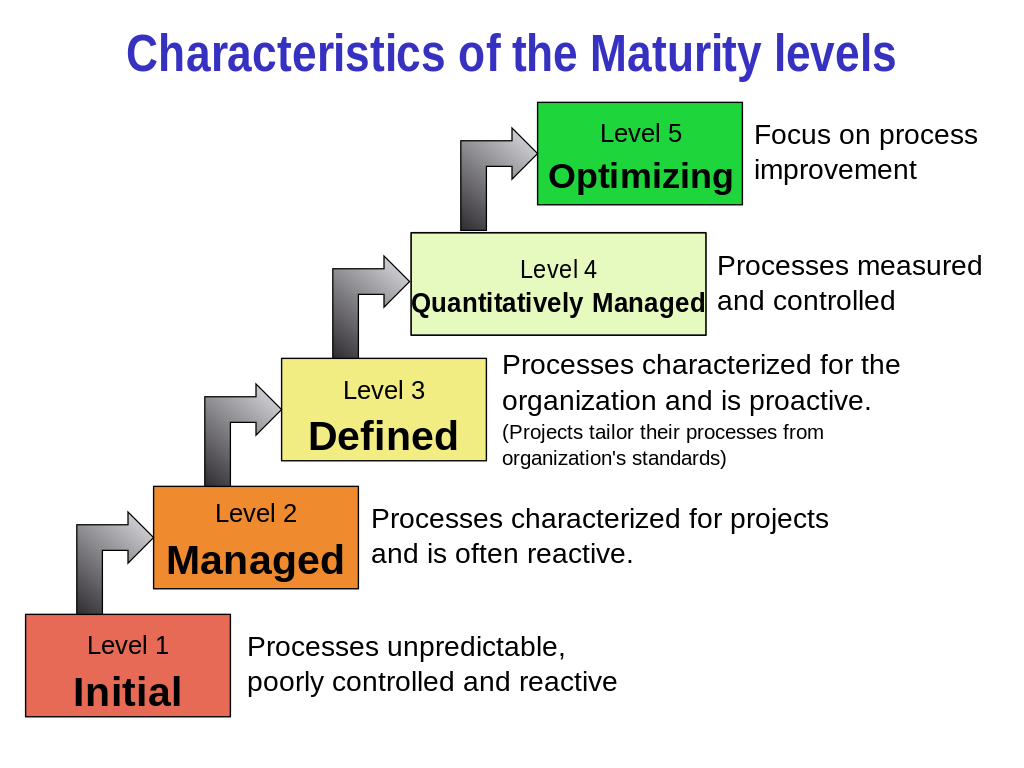
\includegraphics{2C-SE.assets/1024px-Characteristics_of_Capability_Maturity_Model.svg.png}
    \end{itemize}
  \end{itemize}
\item
  \textbf{Total Quality Management (TQM)}

  \begin{itemize}
  \tightlist
  \item
    \textbf{Plan, Do, Check, Act}
  \item
    \emph{Improving quality is everyone's job -\/-not just that of the
    QA department!}
  \end{itemize}

  \begin{enumerate}
  \def\labelenumi{\arabic{enumi}.}
  \tightlist
  \item
    Quality can and must be managed.
  \item
    \emph{Everyone} has a customer to delight.
  \item
    Processes, not the people, are the problem.
  \item
    \emph{Every employee is responsible for quality.}
  \item
    Problems must be \emph{prevented}, not just fixed.
  \item
    Quality must be \emph{measured}, so it can be \emph{controlled}.
  \item
    \emph{Quality improvements must be continuous.}
  \item
    \textbf{Quality goals must be based on customer requirements.}
  \end{enumerate}
\end{itemize}

\begin{itemize}
\tightlist
\item
  \textbf{ISO 9001}

  \begin{itemize}
  \tightlist
  \item
    An international standard for quality assurance.
  \item
    It specifies \emph{how} to specify documents, and procedures that a
    company should follow in its quality control. It \emph{does not}
    however, specify or require any \emph{level of product quality}.
  \end{itemize}
\end{itemize}

\begin{itemize}
\tightlist
\item
  \textbf{Bottom line:} things only get better when those involved...

  \begin{itemize}
  \tightlist
  \item
    ...have enough information to tell what's wrong

    \begin{itemize}
    \tightlist
    \item
      that's why you aim to take \emph{quantitative measurements}
    \end{itemize}
  \item
    ...think about the process

    \begin{itemize}
    \tightlist
    \item
      nothing important, merely stating that you need to know that a
      thing called QA exists
    \end{itemize}
  \item
    ...plan how to improve

    \begin{itemize}
    \tightlist
    \item
      not only the specific product, but the whole process
    \end{itemize}
  \item
    ...actually make sure the plan happens

    \begin{itemize}
    \tightlist
    \item
      quality control
    \end{itemize}
  \item
    ...check whether it worked

    \begin{itemize}
    \tightlist
    \item
      quality control \& quality imprvement
    \end{itemize}
  \end{itemize}
\end{itemize}

\hypertarget{estimating}{%
\paragraph{"Estimating"}\label{estimating}}

\begin{itemize}
\item
  \textbf{Cost estimation}

  \begin{itemize}
  \tightlist
  \item
    Prior to any -\/-significant-\/- project, you need to
    \emph{estimate} how much it will \emph{cost}.

    \begin{itemize}
    \tightlist
    \item
      Time cost, human resources cost, financial cost, ...
    \end{itemize}
  \item
    Many factors:

    \begin{itemize}
    \tightlist
    \item
      software size
    \item
      software complexity
    \item
      engineer productivity (individually and as a team)
    \end{itemize}
  \item
    \textbf{We'll consider only software size and complexity}

    \begin{itemize}
    \tightlist
    \item
      and define \emph{Productivity is the ratio of these to time
      required.}
    \end{itemize}
  \end{itemize}
\item
  \textbf{Lines of Code (LoC)}

  \begin{itemize}
  \tightlist
  \item
    {[}-{]} Not very meaningful by itself, what is a line of code?
  \item
    {[}-{]} Does not make sense across different programming languages:
    imagine Haskell, Java, C...
  \item
    {[}+{]} Still widely used! Alternatives like "function points"
    exist.
  \end{itemize}
\end{itemize}

\hypertarget{estimation-approaches}{%
\subparagraph{\texorpdfstring{\textbf{Estimation
approaches}}{Estimation approaches}}\label{estimation-approaches}}

\begin{itemize}
\item
  \textbf{algorithmic cost modelling} develop (from past data) a model
  relating size/complexity to ultimate cost
\item
  \textbf{expert consensus} get a bunch of expert estimates; compare,
  discuss, and repeat until convergence
\item
  \textbf{analogy} relate the cost to that of similar completed projects
\item
  \emph{\textbf{what customer will pay}} dangerous...
\item
  \textbf{COCOMO I}

  \begin{itemize}
  \tightlist
  \item
    {[}+{]} A long-standing algorithmic model, publicly available, well
    supported and widely used.
  \item
    \$\$ \textbackslash{}text\{Effort\} = \textbackslash{}text\{A\}
    \textbackslash{}times
    \textbackslash{}text\{Size\}\^{}\textbackslash{}text\{B\}
    \textbackslash{}times \textbackslash{}text\{M\} \$\$

    \begin{itemize}
    \tightlist
    \item
      \textbf{Effort} is measured in person-months
    \item
      \textbf{A} is a constant, dependent on kind of software \emph{and}
      developing organisation
    \item
      \textbf{B} typically range in \$\$1\textbackslash{}ldots 1.5\$\$.
    \item
      \textbf{M} is a \emph{multiplier}. Product of 15 factors, each
      typically in range \$0.9\textbackslash{}ldots 1.4\$, that are
      derived from ratings of attributes such as: \emph{required
      reliability}, \emph{required time to market}, \emph{software
      engineer capability}, ...
    \end{itemize}
  \item
    {[}- {]} Getting good values for \textbf{A}, \textbf{B}, and
    \textbf{M} is highly non-trivial.

    \begin{itemize}
    \tightlist
    \item
      {[}+{]} Considerable data available too.
    \end{itemize}
  \item
    Different versions, sub-models, tweaks available.
  \end{itemize}
\end{itemize}

\hypertarget{scheduling}{%
\paragraph{"Scheduling"}\label{scheduling}}

\begin{itemize}
\item
  \textbf{Why do projects almost always slip?}

  \begin{itemize}
  \tightlist
  \item
    \emph{"People tend to be risk-averse when there is a potential of
    loss"}
  \item
    \emph{"People are unduly optimistic in their plans and forecasts"}
  \item
    \emph{"People prefer to use intuitive judgement rather than
    (quantitative) models"}
  \end{itemize}
\item
  \textbf{Gantt Charts}

  \begin{itemize}
  \tightlist
  \item
    Divide project into \textbf{tasks}, with \textbf{milestones} at the
    end.
  \item
    Analyse dependencies between tasks.
  \item
    Lay these tasks out as \textbf{bars running across time},
    \emph{respecting dependencies}.
  \item
    The graph reveals the \textbf{critical path} of tasks for the
    project.
  \item
    Optionally, show \textbf{permissible slippage} with shaded bars.
  \item
    For example:

    \begin{itemize}
    \tightlist
    \item
      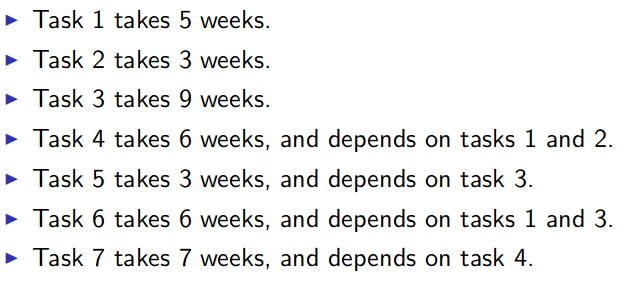
\includegraphics{2C-SE.assets/1543585250853.png}
    \item
      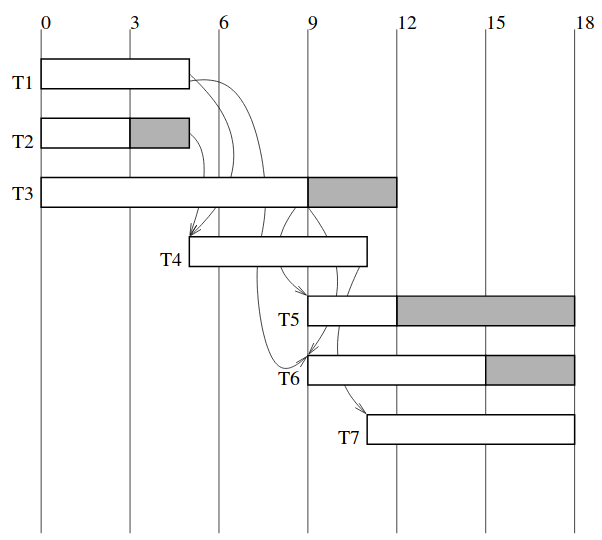
\includegraphics{2C-SE.assets/1543585265509.png}
    \end{itemize}
  \end{itemize}
\end{itemize}

\hypertarget{the-rest}{%
\paragraph{The Rest}\label{the-rest}}

\begin{itemize}
\tightlist
\item
  \textbf{Tracking}

  \begin{itemize}
  \tightlist
  \item
    A balance between too little and too much information to track.

    \begin{itemize}
    \tightlist
    \item
      One is insufficient, one is too much to process and manage!
    \end{itemize}
  \end{itemize}
\item
  \textbf{Revising the Project Plan}

  \begin{itemize}
  \tightlist
  \item
    As the project goes on, estimates have to be revised in the light of
    progress, unforeseen problems, in other words, recent developments!
  \end{itemize}
\end{itemize}

\hypertarget{20-november-2018}{%
\subsection{20 November 2018}\label{20-november-2018}}

\hypertarget{non-functional-requirements-nfr}{%
\subsubsection{Non-Functional Requirements
(NFR)}\label{non-functional-requirements-nfr}}

\begin{itemize}
\tightlist
\item
  \textbf{Concerns the whole system, not just the software}
\item
  About

  \begin{itemize}
  \tightlist
  \item
    Ways the system needs to be related to other system and versions of
    itself:

    \begin{itemize}
    \tightlist
    \item
      flexibility
    \item
      maintainability
    \item
      reusability
    \item
      portability
    \end{itemize}
  \item
    Properties of the system in use

    \begin{itemize}
    \tightlist
    \item
      usability
    \item
      \emph{dependability}

      \begin{itemize}
      \tightlist
      \item
        safety, reliability, availability, resilience
      \end{itemize}
    \item
      \emph{efficiency}

      \begin{itemize}
      \tightlist
      \item
        \emph{performance} (throughput, response time), resource usage
      \end{itemize}
    \item
      \emph{security}

      \begin{itemize}
      \tightlist
      \item
        integrity, confidentiality
      \end{itemize}
    \item
      scalability
    \end{itemize}
  \end{itemize}
\item
  NFRs must be identified along with functional requirements -\/- at the
  end is to late.
\item
  \textbf{Often tied up with architectural decisions} which are almost
  impossible to modify later.
\item
  It is essential to

  \begin{itemize}
  \tightlist
  \item
    \textbf{quantify the requirement}
  \item
    \textbf{have ways to measure -\/- \emph{metrics}}
  \end{itemize}
\end{itemize}

\hypertarget{metrics}{%
\subsubsection{Metrics}\label{metrics}}

\begin{itemize}
\tightlist
\item
  Ideally, metrics are

  \begin{itemize}
  \tightlist
  \item
    \textbf{measurable} not based on "intuition" or "opinions" of
    someone
  \item
    \textbf{specified with a precision} \emph{i.e.} uncertainities must
    be recorded
  \item
    \textbf{MEANINGFUL} numbers must have something to do with something
    we care about!
  \end{itemize}
\end{itemize}

\hypertarget{reliability-metric}{%
\paragraph{Reliability Metric}\label{reliability-metric}}

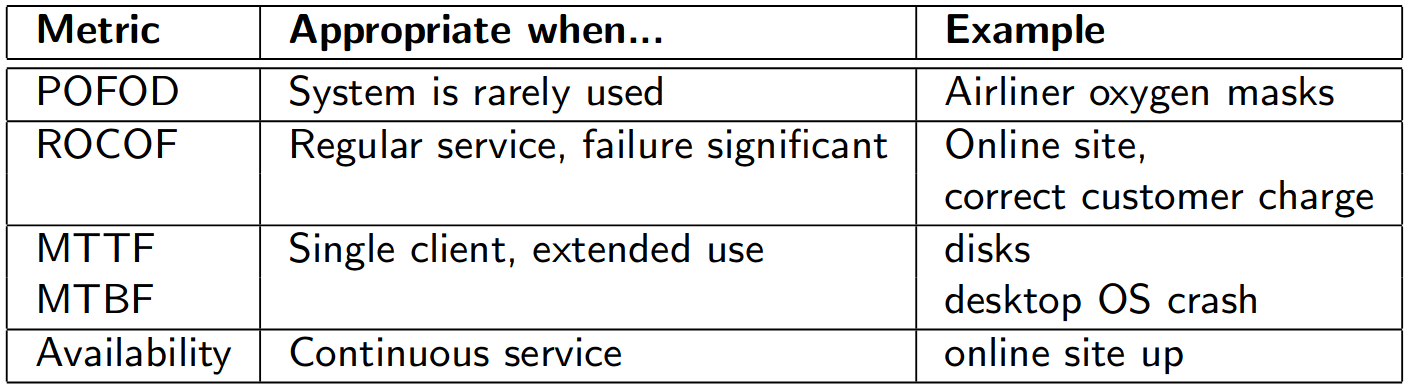
\includegraphics{2C-SE.assets/1543668447275.png}

\begin{itemize}
\tightlist
\item
  \textbf{Reliability is a key non-function requirement in many
  systems.}
\item
  \textbf{There are several ways to specify reliability requirements,
  depending on the nature of the system.}
\end{itemize}

\hypertarget{pofod---probability-of-failure-on-demand}{%
\subparagraph{POFOD - Probability of Failure on
Demand}\label{pofod---probability-of-failure-on-demand}}

\begin{itemize}
\tightlist
\item
  POFOD is the probability that the system will fail when service is
  requested.
\item
  \textbf{Mainly useful for systems that provide emergency or safety
  services.}

  \begin{itemize}
  \tightlist
  \item
    \emph{e.g.} the emergency shutdown in a nuclear power plant will
    (hopefully) never be used -\/- but if it is, it should not fail!
  \end{itemize}
\item
  Can be evaluated through...

  \begin{itemize}
  \tightlist
  \item
    ...repeated tests in simulation.

    \begin{itemize}
    \tightlist
    \item
      which might be expensive.
    \end{itemize}
  \item
    ...static analysis of the whole system

    \begin{itemize}
    \tightlist
    \item
      which is definitely expensive, and to ensure that our analysis is
      correct, some real-world testing would be required.
    \end{itemize}
  \end{itemize}
\end{itemize}

\hypertarget{rocof---rate-of-occurrence-of-failure}{%
\subparagraph{ROCOF - Rate of Occurrence of
Failure}\label{rocof---rate-of-occurrence-of-failure}}

\begin{itemize}
\tightlist
\item
  ROCOF is the number per unit time of failures (\emph{i.e.} unexpected
  behaviour).
\item
  \textbf{Time may mean \emph{elapsed time}, \emph{processing time},
  \emph{Number of Transactions}, \emph{etc.}}
\item
  \textbf{Mainly used for systems providing regular service, where
  failure is significant.}

  \begin{itemize}
  \tightlist
  \item
    \emph{e.g.} banking systems

    \begin{itemize}
    \tightlist
    \item
      VisaNet processes over 10\^{}9\^{} transactions/day. Failure rate
      is not published, but probably (much) less than 10\^{}-5\^{}
      failures/transaction.
    \end{itemize}
  \end{itemize}
\end{itemize}

\hypertarget{mttf--mtbf---mean-time-tobetween-failures}{%
\subparagraph{MTTF \& MTBF - Mean Time To/Between
Failures}\label{mttf--mtbf---mean-time-tobetween-failures}}

\begin{itemize}
\item
  \textbf{MTTF is used when system is non-repairable.}

  \begin{itemize}
  \tightlist
  \item
    \emph{e.g.} often in the case of hardware
  \end{itemize}
\item
  \textbf{MTBF is used when system can recover from failures.}

  \begin{itemize}
  \tightlist
  \item
    \emph{e.g.} operating system crashes
  \end{itemize}
\item
  \textbf{Both are mainly used where a single client uses the system
  \emph{for a long time}.}

  \begin{itemize}
  \tightlist
  \item
    \emph{e.g.} desktop PCs (and their components), \emph{consumer
    products}
  \end{itemize}
\item
  \textbf{Keep in mind that \emph{mean} alone is often insufficient to
  be decisive:}

  \begin{itemize}
  \tightlist
  \item
    Variation matters! 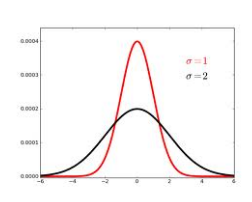
\includegraphics{2C-SE.assets/1543667647524.png}

    \begin{itemize}
    \tightlist
    \item
      Whilst the component whose MTTF is shown with the red curve is
      more predictable to fail after MTTF whilst the blue curve
      indicates that the failure might occur much before (or much after)
      the MTTF.
    \item
      \emph{You would like your curve to be sharp \& pointy.}
    \end{itemize}
  \end{itemize}
\end{itemize}

\hypertarget{availability}{%
\subparagraph{Availability}\label{availability}}

\begin{itemize}
\tightlist
\item
  Availability is the portion of the time that the system is "available
  for use".
\item
  Often quoted as "five nines" (0.99999), "four nines", \emph{etc.}
\item
  \textbf{Appropriate for systems offering a \emph{continuous service},
  where clients expect it to be there all the time.}
\item
  Often achieved by large data processing systems, such as mainframes.
\item
  \textbf{The difference between availability and ROCOF} is that
  availability takes the time to recover from a failure into
  consideration too; \emph{availability gives a better overall picture.}

  \begin{itemize}
  \tightlist
  \item
    For instance your ROCOF might be once in a year, but if it takes you
    3 months to recover, that's not high availability.
  \end{itemize}
\end{itemize}

\hypertarget{usability}{%
\subsubsection{Usability}\label{usability}}

\begin{itemize}
\item
  We'll concern ourselves with User Interfaces (UI) only.
\item
  \emph{Most user errors are actually interface design failures.}
\item
  \textbf{Human Limitations:} Humans...

  \begin{itemize}
  \tightlist
  \item
    ...have very limited short-term memory: 5-7 items.
  \item
    ...make mistakes, especially under stress.
  \item
    ...vary widely, capability-wise, preference-wise, and so on.
  \item
    ...organise their perceived world differently!
  \end{itemize}
\end{itemize}

\hypertarget{principles-of-ui-design}{%
\paragraph{Principles of UI Design}\label{principles-of-ui-design}}

\begin{itemize}
\item
  \textbf{User familiarity}

  \begin{itemize}
  \tightlist
  \item
    The interface should "look familiar" to the users.

    \begin{itemize}
    \tightlist
    \item
      It should use concepts and \emph{entities} (\emph{e.g.} textboxes,
      buttons, sliders) from existing experience of the users.
    \end{itemize}
  \end{itemize}
\item
  \textbf{Consistency}

  \begin{itemize}
  \tightlist
  \item
    Similar operations should be represented in similar ways.

    \begin{itemize}
    \tightlist
    \item
      \emph{E.g.} Red always indicates a situation that requires
      caution, or to draw the user's attention; yellow indicates
      recoverable failure, ...
    \end{itemize}
  \item
    Consistency should be enforced (at least) across the application,
    but many "systems" (Android, iOS, ...) also enforce it across
    \emph{all applications}.

    \begin{itemize}
    \tightlist
    \item
      Brands enforce their own consistency too! Microsoft and Google
      apps look alike across all the platforms.
    \end{itemize}
  \item
    \emph{Beware that similarity might not always be well defined!}
  \end{itemize}
\item
  \textbf{Minimal surprise}

  \begin{itemize}
  \tightlist
  \item
    Avoid situations where the user will be surprised by the behaviour
    of the system.
  \item
    Often is the case with \emph{modal} applications where different
    keys have different effects in different modes.
  \end{itemize}
\item
  \textbf{Recoverability}

  \begin{itemize}
  \tightlist
  \item
    Allow the user to recover (easily) from errors.
  \item
    \emph{Reversibility} (\emph{i.e.} being able to undo) is relevant
    here.
  \item
    Checkpointing/autosaving is a valuable technique.
  \end{itemize}
\item
  \textbf{User guidance}

  \begin{itemize}
  \tightlist
  \item
    Kindly guide the user for taking the appropriate action through your
    UI.

    \begin{itemize}
    \tightlist
    \item
      As opposed to demanding them read 100 pages long manual.
    \end{itemize}
  \item
    Provide \emph{meaningful} (\emph{i.e.} actionable) error messages.

    \begin{itemize}
    \tightlist
    \item
      \emph{E.g.} Bad: "File Save Error" Good: "File could not be saved
      because disk is full; open up some space and try again."
    \item
      This is not always easy of course, there are tons of assumptions
      we make within our abstractions which -\/-when violated-\/- does
      not yield a meaningful error message.
    \end{itemize}
  \end{itemize}
\item
  \textbf{User diversity}

  \begin{itemize}
  \tightlist
  \item
    Remember that users vary on numerous levels on various axes.

    \begin{itemize}
    \tightlist
    \item
      Healthy, colour-blind, blind
    \item
      Healthy, hearing-impaired, deaf
    \item
      Fluent in English, intermediate, doesn't know English, or even
      illiterate!
    \item
      Power users, casual users
    \end{itemize}
  \item
    Wherever possible, provide choices for \emph{customisability}.
  \item
    Often there are legal obligations about \emph{accessibility}.
  \end{itemize}
\end{itemize}

\hypertarget{task-analysis}{%
\paragraph{Task Analysis}\label{task-analysis}}

\begin{enumerate}
\def\labelenumi{\arabic{enumi}.}
\tightlist
\item
  What tasks users want to do with the system?
\item
  In what order and combination?
\end{enumerate}

\begin{itemize}
\tightlist
\item
  \emph{E.g.} Information should be presented wherever it is required.

  \begin{itemize}
  \tightlist
  \item
    AND to reduce the clutter, \emph{information should not be
    represented wherever it is not required.}
  \end{itemize}
\item
  Running through user stories and use cases are often useful here.
\end{itemize}

\hypertarget{user-interaction}{%
\paragraph{User Interaction}\label{user-interaction}}

\begin{itemize}
\item
  How do users interact with the system?
\item
  \textbf{Direct manipulation} such as drag-and-drop
\item
  \textbf{Menu selection} perhaps on a directly selected object
\item
  \textbf{Form fill-in} typically used for data entry
\item
  \textbf{Command language} typically used by traditional systems (UNIX)
\item
  \textbf{Natural language} sometimes as a front end to a command
  language, but more advanced versions have emerged such as Siri, using
  NLP
\item
  \textbf{Body language} such as Nintendo Wii, or XBox Kinect
\end{itemize}

\hypertarget{information-presentation}{%
\paragraph{Information Presentation}\label{information-presentation}}

\begin{itemize}
\item
  How should information be presented to the user?

  \begin{itemize}
  \tightlist
  \item
    This has \emph{nothing} to do with the way information is
    represented internally.
  \end{itemize}
\item
  Continuously varying information is best represented in an analogue
  representation (\emph{i.e.} continuous graphs), not as numbers.

  \begin{itemize}
  \tightlist
  \item
    \emph{Data visualisation}
  \end{itemize}
\item
  \textbf{Presentation should depend on the audience: \emph{e.g.} graphs
  vs graphics.}
\end{itemize}

\hypertarget{colour}{%
\paragraph{Colour}\label{colour}}

\begin{itemize}
\tightlist
\item
  Use few colours \emph{consistently}, no more than four or five per
  context and no more than seven in total.
\item
  Colour changes should signal something significant.
\item
  Be careful about colour pairings (\emph{e.g.} do not put red on blue
  background).

  \begin{itemize}
  \tightlist
  \item
    Contrast also affects accessibility; low contrast is harder to
    process visually (in general, but especially for the visually
    impaired).
  \end{itemize}
\item
  In general, vary colours along only one of the three dimensions (hue,
  saturation, brightness) to make a distinction.
\item
  Know the output technology; primary green is often unreadable on
  screen but fine in print.
\item
  Remember that around 10\% of men are red-green colour-blind!
\end{itemize}

\hypertarget{interface-design-and-evaluation}{%
\paragraph{Interface design and
evaluation}\label{interface-design-and-evaluation}}

\begin{itemize}
\tightlist
\item
  Design iteratively.
\item
  Only real end users are good judges of the interface; testing is
  important.

  \begin{itemize}
  \tightlist
  \item
    Evaluation is hard; get professionals, read HCI books.
  \end{itemize}
\item
  In expensive or critical software, involve professional from
  appropriate fields (\emph{e.g.} ethnography).
\end{itemize}

\hypertarget{22-november-2018}{%
\subsection{22 November 2018}\label{22-november-2018}}

\hypertarget{intellectual-property-ip}{%
\subsubsection{Intellectual Property
(IP)}\label{intellectual-property-ip}}

\begin{quote}
IP is not property, and it's not intellectual. It resists definition,
but one definition of IP might be: \emph{a monopoly right to exploit an
intangible product of human thought or labour.}
\end{quote}

Several broad categories:

\begin{itemize}
\tightlist
\item
  \textbf{copyright} applies to literary or artistic works
\item
  \textbf{patents} apply to inventions of things or processes
\item
  \textbf{design rights} apply to design of products
\item
  \emph{none of these were invented with software in mind...}
\end{itemize}

\hypertarget{patents}{%
\paragraph{Patents}\label{patents}}

\begin{itemize}
\tightlist
\item
  Arose to protect \emph{inventors} of physical objects or processes.
\item
  \textbf{Stronger than copyright}

  \begin{itemize}
  \tightlist
  \item
    stops other people using/making object even if they invented it
    independently
  \end{itemize}
\item
  \textbf{Duration is sorter} -\/- 17 years
\item
  \textbf{Software patents are controversial}

  \begin{itemize}
  \tightlist
  \item
    In U.S., yes; in Europe, no (roughly speaking).
  \item
    In U.S., \emph{business processes} are patentable (\emph{e.g.}
    Amazon has patents on \emph{one-click} shopping, and on the idea of
    customers reviewing products!).
  \end{itemize}
\end{itemize}

\hypertarget{copyright}{%
\paragraph{Copyright}\label{copyright}}

\begin{itemize}
\item
  Copyright protects \emph{the expression of an idea}, not the idea
  itself.

  \begin{itemize}
  \tightlist
  \item
    \emph{The original IP.}
  \end{itemize}
\item
  Restricts the ability to copy, adapt, \emph{etc.} artistic or literary
  works.
\item
  \textbf{Unlike patents, no merit {[}invention{]} is required; this
  document is a literary work for copyright purposes.}
\item
  \textbf{Duration is longer} -\/- life of author + \textasciitilde{}70
  years.
\item
  \textbf{The protected rights may be \emph{assigned} in whole or in
  part, or \emph{licensed} in whole or in part, with or without
  restrictions.}
\item
  Source code is subject to copyright.

  \begin{itemize}
  \tightlist
  \item
    Object code and machine code are \emph{adaptations or translations}
    of source code, hence protected.
  \end{itemize}
\item
  Clean-room reverse engineering is permissible under many
  jurisdictions.
\end{itemize}

\hypertarget{licenses}{%
\paragraph{Licenses}\label{licenses}}

\begin{itemize}
\tightlist
\item
  Can be licensed per computer, per user, or per CPU cores!
\item
  Sometimes it's the license to access and use a website.

  \begin{itemize}
  \tightlist
  \item
    \emph{E.g.} Office 365
  \end{itemize}
\item
  Shareware/Fremimum, Free Open Source, Proprietary, ...
\item
  GPL -\/- General Public License

  \begin{itemize}
  \tightlist
  \item
    \textbf{copyleft} -\/- modifications or adaptations of the work
    (including other works which depends on it) must be licensed under
    the same license.
  \item
    As a result, \emph{copyleft licenses are incompatible with each
    other}.
  \end{itemize}
\item
  LGPL -\/- Lesser General Public License

  \begin{itemize}
  \tightlist
  \item
    \textbf{weak copyleft} -\/- same as GPL, except other works which
    depends on our work does \emph{not} have to be licensed under the
    same license.
  \item
    Again, incompatible with other copyleft licenses.
  \end{itemize}
\end{itemize}

Choosing a license may depend on:

\begin{itemize}
\tightlist
\item
  \textbf{philosophy} some consider restricting software to be
  unethical, some motivated by utilitarian views...
\item
  \textbf{legal constraints} you may have used other software that
  restricts your choices (proprietary or copyleft).
\item
  \textbf{business relevance} sharing the most valuable asset of your
  company might not be the best business strategy!
\item
  \textbf{support} do you want your users to contribute?
\end{itemize}

\hypertarget{27-november-2018}{%
\subsection{27 November 2018}\label{27-november-2018}}

\hypertarget{ethics}{%
\subsubsection{Ethics}\label{ethics}}

\begin{quote}
Software engineers shall commit themselves to making the analysis,
specification, design, development, testing and maintenance of software
a \emph{beneficial} and respected profession. In accordance with their
commitment to the health, safety and welfare of the public, software
engineers shall adhere to the following Eight Principles:

\begin{enumerate}
\def\labelenumi{\arabic{enumi}.}
\tightlist
\item
  \textbf{PUBLIC} -\/-\/- Software engineers shall act consistently with
  the public interest.
\item
  \textbf{CLIENT AND EMPLOYER} -\/-\/- Software engineers shall act in a
  manner that is in the best interests of their client and employer
  consistent with the public interest.
\item
  \textbf{PRODUCT} -\/-\/- Software engineers shall ensure that their
  products and related modifications meet the highest professional
  standards possible.
\item
  \textbf{JUDGEMENT} -\/-\/- Software engineers shall maintain integrity
  and independence in their professional judgement.
\item
  \textbf{MANAGEMENT} -\/-\/- Software engineering mangers and leaders
  shall subscribe to and promote an ethical approach to the management
  of software development and maintenance.
\item
  \textbf{PROFESSION} -\/-\/- Software engineers shall advance the
  integrity and reputation of the profession consistent with the public
  interest.
\item
  \textbf{COLLEAGUES} -\/-\/- Software engineers shall be fair to and
  supportive of their colleagues.
\item
  \textbf{SELF} -\/-\/- Software engineers shall participate in lifelong
  learning regarding the practice of their profession and shall promote
  an ethical approach to the practice of the profession.
\end{enumerate}
\end{quote}

\href{https://ethics.acm.org/code-of-ethics/software-engineering-code/}{https://ethics.acm.org/code-of-ethics/software-engineering-code/}

\begin{itemize}
\tightlist
\item
  \textbf{You should be able to answer, given an example, which codes of
  ethics the incident violates.}
\end{itemize}

\end{document}
